
\documentclass[12pt]{report}
\usepackage{fancyhdr}
\usepackage[a4paper, margin=1in]{geometry}
\usepackage{graphicx}
\usepackage{fancyhdr}
\usepackage{titlesec}
\usepackage{tocloft}
\usepackage{setspace}
\usepackage{caption}
\usepackage{float}
\usepackage{longtable}
\usepackage{lipsum}
\usepackage{amsmath}
\usepackage{enumitem}
\usepackage{array}
\usepackage{tabularx}
\usepackage{needspace}
\usepackage{adjustbox}
\usepackage[utf8]{inputenc}

% ----- Fix uneven word spacing -----
\usepackage{microtype}       % Smooths word/letter spacing
\sloppy                      % Prevents over-tight spacing
\emergencystretch=3em        % Prevents stretched/ugly lines

% ----- Remove extra space after punctuation -----
\frenchspacing

\renewcommand{\arraystretch}{1.4}
\setlength{\tabcolsep}{6pt}
\setlength{\parindent}{0pt}
\setlength{\parskip}{6pt}
\onehalfspacing

% Hyperref
\usepackage[
    backref=page,
    colorlinks=true,
    linkcolor=black,
    filecolor=black,
    urlcolor=blue,
    citecolor=blue
]{hyperref}

% Backref Formatting
\renewcommand*{\backref}[1]{}
\renewcommand*{\backrefalt}[4]{%
  \ifcase #1 %
  \or
    (Cited on p.~#2)%
  \else
    (Cited on pp.~#2)%
  \fi
}

\begin{document}

% ---------------- Title Page ----------------
\begin{titlepage}
\pagenumbering{roman}
\centering
\vspace*{1cm}

{\LARGE \textbf{Wheel Share App}}\\[2cm]


\includegraphics[width=6cm]{BUI-Logo.jpg}\\[2cm]

Izzah Malik\\
\textbf{01-135211-039}\\[0.5cm]
Umair Khan\\
\textbf{01-135212-096}\\[1.5cm]


Supervisor: Syed Junaid Hussain\\[1.5cm]

{\large \textbf{Bachelor of Science in Information Technology}}\\[0.5cm]
Department of Computer Science\\
Bahria University, Islamabad\\[0.5cm]
December 2025


\vfill
\end{titlepage}



% ---------------- Certificate ----------------
\chapter*{\centering Certificate}
\addcontentsline{toc}{chapter}{Certificate}

We acknowledge the work presented in the report titled \textbf{Wheel Share App}, authored by Ms. Izzah Malik and Mr. Umair Khan, as meeting the required standards for the partial fulfillment of the Bachelor of Science in Information Technology degree.\\[1.2cm]

\textbf{Approved by:}\\[0.2cm]

Supervisor: Syed Junaid Hussain\\
\noindent\makebox[\textwidth]{\hrulefill}\\[0.2cm]

Internal Examiner: Name of the Internal Examiner (Title)\\
\noindent\makebox[\textwidth]{\hrulefill}\\[0.2cm]

External Examiner: Name of the External Examiner (Title)\\
\noindent\makebox[\textwidth]{\hrulefill}\\[0.2cm]

Project Coordinator: Dr. Kabeer Ahmed Bhatti\\
\noindent\makebox[\textwidth]{\hrulefill}\\[0.2cm]

Head of Department: Dr. Muhammad Khurram Ehsan\\
\noindent\makebox[\textwidth]{\hrulefill}\\[0.2cm]

\textbf{December 15th, 2025}

\clearpage

% ---------------- Abstract ----------------
\chapter*{Abstract}
\addcontentsline{toc}{chapter}{Abstract}

Wheel Share is a Flutter-based ride-sharing program that links drivers and riders going to comparable locations. It is powered by Supabase (PostgreSQL). Through shared trips, it encourages economical, convenient, and environmentally responsible transportation. The two main roles the application offers are Driver and User. While drivers may post rides, manage earnings, and accept offers, users can search for rides, issue offers, and monitor spending. Important components include an admin panel for monitoring rides, users, and alerts, ratings and reviews for trust, and an emergency alert system for safety. Wheel Share’s cross-platform functionality, secure authentication, and real-time updates make it a dependable and scalable solution for smart urban mobility, reducing traffic and promoting sustainable transportation.

% ---------------- Acknowledgement ----------------
\chapter*{Acknowledgement}
\addcontentsline{toc}{chapter}{Acknowledgement}

We are incredibly appreciative of Allah Almighty, the Most Merciful and Beneficent, for all His bounties during our academic careers. We are deeply grateful to our supervisor, Syed Junaid Hussain, for his important advice, steadfast support, and helpful criticism, all of which were essential to this project's successful conclusion. We would like to express our sincere gratitude to our parents, whose unwavering support and prayers made this accomplishment possible, as well as to our family and friends, who have always been a source of inspiration. We also thank Bahria University’s Department of Computer Science for providing a helpful learning environment. The support we have received from everyone is reflected in this initiative.

\vspace{4\baselineskip}

Izzah Malik, Umair Khan\\
Islamabad, Pakistan

\clearpage

% ---------------- Quote Page ----------------
\vspace*{\fill}
\begin{center}
\textit{“Learning is the spark that ignites change in the world.”}\\
\hfill -- Malala Yousafzai
\end{center}
\vspace*{\fill}
\clearpage

% ---------------- TOC ----------------
\tableofcontents
\clearpage
\listoffigures
\clearpage
\listoftables
\cleardoublepage

% ---------------- Acronyms and Abbreviations ----------------
\chapter*{Acronyms and Abbreviations}
\addcontentsline{toc}{chapter}{Acronyms and Abbreviations}

\vspace{1cm}

\begin{tabbing}
\hspace{4cm}\=\hspace{8cm}\=\kill

\textbf{JWT} \> JSON Web Token \\
\textbf{API} \> Application Programming Interface \\
\textbf{GUI} \> Graphical User Interface \\
\textbf{UI} \> User Interface \\
\textbf{VS Code} \> Visual Studio Code \\
\textbf{IDE} \> Integrated Development Environment \\
\textbf{RSL} \> Ride Sharing Layer \\
\textbf{Supabase SQL} \> Supabase Structured Query Language \\
\end{tabbing}
\clearpage
\pagenumbering{arabic}

% ================= Chapter Header Setup =================

\pagestyle{fancy}

% Clear all headers/footers
\fancyhf{}

% Remove header rule on all pages by default
\renewcommand{\headrulewidth}{0pt}

% Define custom chapter mark
\renewcommand{\chaptermark}[1]{%
  \markboth{CHAPTER \thechapter\ -- #1}{}}

% Right header (ONLY from page 2 of chapter)
\fancyhead[R]{\leftmark}

% Page number center footer
\fancyfoot[C]{\thepage}

% First page of each chapter (plain style)
\fancypagestyle{plain}{
  \fancyhf{}
  \renewcommand{\headrulewidth}{0pt}
  \fancyfoot[C]{\thepage}
}
% ========================================================



% ---------------- Chapters ----------------
\chapter{Introduction}
The increasing interest in sustainable modes of transport and cost effective commuting has motivated the creation of grand ride-sharing concepts in the global context. Wheel Share is a community-based priority ride-sharing system which offers a secure, scalable, and easy experience to customers and the passengers who travel in the same direction. Will using Flutter as the frontend and Supabase (PostgreSQL) as the backend and Google API for location. The system promotes car sharing that saves gas and amounts of traffic growth, traffic congestion and encourage the sustainability of the environment. Ride-Sharing in a period when gas prices are increasing and where the issue of environmental awareness is on the rise.
Ride-Sharing has turned to be a viable and greener way of transport. However, most existing ride sharing services are commercialized and have high commissions, which makes it community-based, affordable and centralized alternative. Through this platform, users can is used in order to post available rides.
Passenger can also search for and send offers to join.
In is also provided on the platform built in controls on financial overviews, rating schemes on critiques, and an emergency option which guaranties safety of the user.
It uses cross platform flexibility of Flutter and Supabase real time backend services, Wheel Share makes data management and communication transparent as well as reliable and efficient performance. It does not only create trust and user-to-user collaboration, but it also
is part of the overall objective of sustainable shared mobility
\cite{mitropoulos2021}.


\section{Background}

Transportation remains a daily challenge for millions of individuals, especially in urban areas where congestion, fuel prices, and time delays create significant inconvenience. The idea of carpooling or ride sharing emerged to address these issues by allowing people traveling in the same direction to share a single vehicle, thereby reducing costs and emissions. However, the local communities, in spite of the introduction of the ride sharing services into the global community. We already do not have easy access to low-cost and safe prospects that can address their needs. These challenges have been such that Wheel Share has been created to handle them. The project integrates current mobile and web technologies to turn drivers and a flawless  experience as well for passengers. The user can create profiles, add rides, search, since it has a user-friendly interface to match in journeys, make and receive offers. Both user type, two types of drivers, passenger and administrator is a role that occurs, which has both role and access privileges to assure ordered functionality and data security.
Moreover, it has the emergency alert system, rating, review and capabilities.The earnings spending dashboards also help individuals save time and money besides offering assurance to the users. Wheel Share will,therefore, be a revolution a change of commuting culture to a more ecological and intermediate kind.


\section{Objective}

It will aim at providing a safe convenient along with reliable car-pooling environmentment by integrating the real time communication, open financial track and security features.The main aims will be the creation of a system that will provide the driver and the passengers with the opportunity to communicate and operate rides effectively and with the aim of developing trust, provide feedbacks in a smooth manner\cite{ashkrof2022}. It also dedicated to the empowerment of the users and providing them with the entire control over their rides and trade, and at the same time enable administrators to trace activities and ensure that the platform possesses integrity.

Lastly, Wheel Share will target combination of convenience, cost efficiency and security, provide-
Development of the alternative to the traditional commuting which will be a win-win to the users and the environment.


\section{Problem Description}

Numerous low-cost modes of transportation are being used as a result of the rising need for affordable, effective travel and transportation.Travel costs, expensive forms of transportation, and lack of reliable car-sharing services are all things that people dislike. The market offers a wide range of solutions.The data is heavy, commercial, or geographically restricted, making it impractical for personal or community use.User comments and market observations can help identify some of these.
Through market observation and user feedback, several core issues were identified:


\begin{enumerate}[label=\roman*.]
    \item Lack of localized, affordable ride sharing solutions tailored to community use.
    \item Absence of a transparent system that allows users to view and compare rides based on city, address, and date.
    \item Inadequate financial tracking and transaction monitoring between drivers and passengers.
    \item Safety concerns due to insufficient identity verification and lack of emergency protocols.
    \item Lack of comprehensive dashboards to analyze travel spending and earnings performance.
    

\end{enumerate}


\section{Project Objectives}
The Wheel Share project has been designed with a clear set of objectives to ensure effective implementation and user satisfaction. The objective is to develop a cross-platform mobile application using Flutter that connects drivers and passengers in an efficient, secure, and transparent manner.

The system intends to implement role-based authentication through Supabase to ensure that each user type driver, passenger, and admin has specific access rights and responsibilities. Drivers will be able to post available rides with relevant details and manage offers from users. Passengers will be able to search for rides by city, address, and date, send offers, and manage accepted rides. Additionally, both parties will have access to dashboards that summarize earnings and expenses respectively, helping them maintain financial clarity.

Another key objective is the incorporation of a rating and review system that fosters accountability and builds trust among users. The inclusion of an emergency feature enhances safety by allowing users to alert the admin in case of unforeseen circumstances\cite{gangadharaiah2023}. The admin panel provides tools to monitor user activity, manage rides, handle emergencies, and remove inappropriate users or content.

Together, these objectives ensure that Wheel Share becomes a holistic and user driven platform that encourages shared mobility while maintaining transparency, safety, and convenience.



\section{Project Scope}

The production of a ride sharing application is part of the Wheel Share combines safe authentication, tools of managing and communication cohesive system. The project will be directed at providing a stable platform that contributes to provision posting of rides, searching and managing and ensuring that it is safe and transparent to all users.
The system has three modules namely driver, passenger and administrator. The driver module provides their users with a chance to post rides, offers, and track it, view, and access their ride history. The passenger module allows the ride searching to take place and offers an offer dispatching, and cost tracking. The administration module provides management functionality, monitoring of processes on the platform and management of emergencies and the efficient work of the operation of the system. The user interface is Flutter and the Database and Authentication is Supabase services, Wheel Share will offer data synchrony, data reliability and data efficiency at real time. The concept of analysing it, in the end, all gives to the ride it has made a ride that is both community based and functional Sharing application that promotes price effectiveness, safety and sustainability.
In conclusion, Wheel Share system is capable of realizing the recent technology and community partnership that will provide the new generation, dependable, and green ride-sharing solution. Helping to establish trustful relations and open transactions, and it enhances the experience of commuting to the entirety and generates the commuting experience and 
tend to smarter and better networked cities.


\section{Solution Application Areas}

The Wheel Share system is designed to serve a wide range of users who seek affordable and reliable commuting options. It provides an intelligent ride sharing platform suitable for daily commuters, students, employees, and individuals seeking intercity travel options. The system can be applied in both urban and suburban contexts, where it enables users to share rides, reduce travel expenses, and optimize vehicle usage.

The application also provides significant benefits for environmental sustainability, as it reduces traffic congestion and lowers carbon emissions through shared mobility. Its role-based dashboards empower different stakeholders drivers, passengers, and administrators by providing access to relevant tools and data insights\cite{soria2021}. For drivers, the platform acts as an earnings management tool, while passengers benefit from transparency in travel spending. Administrators can utilize the platform to monitor safety alerts, manage user activities, and ensure smooth operational flow.


\section{Risk Involved}

\subsection{Technical Challenges}
One significant technical challenges in creating Wheel Share is guaranteeing scalability and performance efficiency. The system needs to handle a high volume of ride data while ensuring real-time synchronization among numerous users. Possible risks include problems with integrating Supabase, performance lags in Flutter interfaces, and difficulties in handling multiple concurrent user sessions. These technical challenges, if not swiftly addressed, could affect system reliability and user satisfaction.Therefore, proactive testing, code refinement, and a strong backend design are essential to reduce technical risks.

\subsection{User Adoption}
Another risk is the user adoption. Ride-sharing in which the communication is a significant aspect is also of importance.The most important secret of success is participation that involves the amount of users. Without proper marketing and awareness, the platform will have low participation of drivers or passengers. Local promotions, strategic outreach programs to control this and referrals as incentives can also help to improve the uptake and continued usage of the Wheel Share application
\cite{compostella2025}.

\subsection{Legal Compliance}
The project must also be able to meet the requirements of laws of transportation and data privacy at regional level.Confidence of the legislation of the check of users, protection of data and ride sharing policies should be introduced to avoid the potential legalization. Moreover, maintaining the field of transparency in user identity check and ride histories will help the platform to achieve control and earn customer trust.

 
\clearpage





\chapter{Literature Review}
\section{Ride-Sharing Systems}

One of the most revolutionary developments in urban mobility is ride-sharing, which is changing the way people commute by allowing travelers on comparable routes to share a vehicle. Mitropoulos et al. (2021) claim that ride-sharing services act as a middleman between drivers and passengers, providing economical and ecologically friendly travel options while resolving issues with pollution and urban congestion\cite{mitropoulos2021}.

Alonso-González et al. (2020) looked at the elements that influence users' propensity to share rides and discovered that social comfort, cost savings, journey time, and privacy all have a significant impact on participation decisions\cite{alonso2020}. In a similar vein, Gangadharaiah et al. (2023) introduced the Pooled Rideshare Acceptance Model (PRAM), highlighting the importance of convenience, perceived safety, and trust for the long-term uptake of ridesharing services\cite{gangadharaiah2023}.

Even though ride-sharing services like Uber, Lyft, and BlaBlaCar have their benefits, they frequently work under centralised commercial frameworks that put making money first through commissions and spike pricing.Ashkrof et al. (2022) noted that driver acceptance and behavior toward ride offers are also influenced by dynamic pricing and operational flexibility\cite{ashkrof2022}.


\subsection{User Factors and Barriers in Ride-Sharing Adoption}
A major body of research highlights user psychology and behavioral factors as critical determinants in ride-sharing adoption. Merat et al. (2017) examined the human factors and user acceptance challenges in ride sharing, particularly for automated and digitalized vehicles, noting that perceived control and safety significantly influence user willingness to participate \cite{merat2017}.

Abouelela et al. (2022) found that the frequency of pooled versus solo ride-hailing use depends on demographic characteristics, trip purpose, and time flexibility\cite{abouelela2022}. Dastani et al. (2024) extended this by proposing a mathematical model that integrates transfer convenience, waiting time, and social comfort into ride-sharing preference predictions\cite{dastani2024}.

Participation in ride-sharing is also influenced by social and geographic differences. Users in low-income or less digitally connected neighbourhoods are less likely to use pooled ride-hailing, according to Soria and Stathopoulos (2021), underscoring the significance of equitable design in mobility platforms\cite{soria2021}. According to Compostella et al. (2025), future driverless and automated ride-sharing scenarios will increase consumer perceptions of safety, control, and comfort\cite{compostella2025}.


\subsection{Passenger Safety }
Adoption of ride-sharing is still heavily influenced by safety concerns. According to Chaudhry et al. (2018), ride-sharing systems should have emergency warning capabilities, user rating systems, and identity verification to guarantee accountability since passenger safety is a major factor in determining trust and retention\cite{chaudhry2018}.
Similarly, Acheampong et al. (2021) emphasized that digital mobility platforms should incorporate transparent user data handling and behavioral monitoring to mitigate risks related to harassment, fraud, and privacy breaches\cite{acheampong2021}. 

According to Mageto et al. (2025), users' propensity to utilise ride-hailing services is greatly reduced by perceived hazards, such as a lack of driver screening and ambiguity about route safety. The design of Wheel Share, which has an emergency feature, user authentication system, and rating and review systems to promote community trust and safety, is directly influenced by these insights
\cite{mageto2025}.

\subsection{Trust Mechanisms in Ride-Sharing}
Hussain et al. (2025) explored commuters’ preferences for future ride-sharing and concluded that a combination of safety assurance, technological reliability, and social responsibility drives long-term engagement\cite{hussain2025}.

\subsection{Technological Advancements in Ride-Sharing Systems}
In terms of scalability, accessibility, and real-time response, emerging technologies have completely changed how ride-sharing systems are implemented. According to Taiebat et al. (2022), data-driven insights can optimize matching and pricing algorithms by analyzing user behavior and predicting ride-sharing preferences using machine learning models\cite{taiebat2022}.

In order to promote justice while maintaining platform operations, Bujak and Kucharski (2024) emphasised the significance of striking a balance between profit and traveler acceptance in ride-pooling through customised fare schemes. This idea can be used to community-oriented systems like Wheel Share
\cite{bujak2024}.

\subsection{Automated Ride Monitoring & Safety Insights}
In 2023, R. Taylor et al. presented the Experian Hunter system, originally designed to analyze large datasets and identify unusual patterns. In a ride-sharing context, similar analytical techniques can help understand user behavior,improve platform reliability, and support better decision making while ensuring data privacy and security\cite{taylor2023}.


\subsection{Experian Hunter}
The Experian Hunter system, a data-driven analytical tool initially created to evaluate and analyse massive data sets for anomalous patterns, was introduced by R. Taylor et al. in 2023. Similar analytical techniques can be applied to a ride-sharing setting to examine ride patterns, user activity, and platform interactions in order to guarantee consistency, boost operational effectiveness, and facilitate trustworthy decision-making\cite{taylor2023}. These tools assist ride-sharing services improve service quality and uphold operational and data protection regulations by offering immediate insights and predictive capabilities. 


\subsection{Intelligent Ride Pattern Monitoring}
In 2025, J. Smith et al. discussed the Actimize system, which uses artificial intelligence and predictive analytics to identify unusual patterns and optimize operational decision making\cite{smith2025}. Similar AI-based analytical techniques can be adapted for ride-sharing platforms to improve user safety, ensure reliable matching, and strengthen overall platform trust.
By analyzing behavioral patterns including unusual ride cancellations, duplicate ride postings, or repeated payment disputes predictive models can identify potential misuse or suspicious activity. Real-time alerts and automated risk scoring can then notify administrators for early intervention.

\subsection{FICO Falcon Fraud Manager}
n 2022 A.Lee et al enhanced that FICO Falcon Fraud Manager operates through machine learning to analyze insurance payments for detecting irregular patterns through its artificial intelligence capabilities. Insured party conduct data alongside existing claim statistics combined with payment documents allows FICO Falcon Fraud Manager to discover potential fraudulent activities. Insurers benefit from real-time fraud detection through the system which develops security systems and minimizes false claims by offering data-based choices to reduce insured losses\cite{lee2022}.


\subsection{ClearSale}
In 2019 B. Johson et al presented that ClearSale combines artificial intelligence with human expertise to use its fraud prevention platform for insurance claims verification so it can stop fraudulent activities. Machine learning algorithms analysis within the platform examines claims data to discover system abnormalities that result in assessment report generation. The user-invoked review process improves both fraud detection quality and enables rapid and seamless handling of genuine claims\cite{johnson2019}.

\subsection{Comparison Table}

\renewcommand{\arraystretch}{1.3}
\setlength{\tabcolsep}{4pt}
\small

\begin{longtable}{|c|c|l|
>{\raggedright\arraybackslash}p{3.2cm}|
>{\raggedright\arraybackslash}p{3.5cm}|
>{\raggedright\arraybackslash}p{3.5cm}|}


\hline
\textbf{Ref} & \textbf{Year} & \textbf{Author(s)} &
\textbf{Approach} & \textbf{Contribution} & \textbf{Limitation} \\
\hline
\endfirsthead

\hline
\textbf{Ref} & \textbf{Year} & \textbf{Author(s)} &
\textbf{Approach} & \textbf{Contribution} & \textbf{Limitation} \\
\hline
\endhead

\hline
\multicolumn{6}{r}{\textit{Continued on next page}} \\
\hline
\endfoot

\hline
\endlastfoot

\cite{mitropoulos2021} & 2021 & Mitropoulos et al. &
Study of ride-sharing’s role in urban mobility &
Highlights cost effectiveness and environmental benefits of shared commuting &
Limited focus on safety and trust mechanisms \\ \hline

\cite{alonso2020} & 2020 & Alonso-González et al. &
Behavioral analysis of ride-sharing adoption &
Identifies cost, time, and privacy as key adoption factors &
Does not address fraud or security issues \\ \hline

\cite{gangadharaiah2023} & 2023 & Gangadharaiah et al. &
Pooled Rideshare Acceptance Model (PRAM) &
Establishes safety, trust, and convenience as central to adoption &
Focused mainly on user perception, not implementation \\ \hline

\cite{chaudhry2018} & 2018 & Chaudhry et al. &
Passenger safety in digital mobility &
Proposes safety and emergency alert mechanisms for trust building &
Does not consider real-time fraud or misuse detection \\ \hline

\cite{acheampong2021} & 2021 & Acheampong et al. &
Data transparency and accountability in ride-sharing &
Promotes secure data handling and user behavior monitoring &
Focus limited to privacy rather than fraud prevention \\ \hline

\cite{taylor2023} & 2023 & R. Taylor et al. &
Experian Hunter automated Ride Monitoring &
Safety insights analytics for real-time risk assessment &
Initially designed for safety; needs adaptation for ride-sharing data \\ \hline

\cite{smith2025} & 2025 & J. Smith et al. &
Intelligent ride pattern monitoring and predictive analytics &
Detects anomalies through behavioral and transactional data patterns &
Industry-specific model; lacks mobility-related parameters \\ \hline

\cite{lee2022} & 2022 & A. Lee et al. &
FICO Falcon Fraud Manager using machine learning &
Provides real-time analysis of payment irregularities &
Limited to financial datasets; not optimized for ride-sharing context \\ \hline

\cite{johnson2019} & 2019 & B. Johnson et al. &
ClearSale AI and human review hybrid model &
Enhances fraud detection accuracy through human-in-the-loop verification &
Dependent on manual review, which may reduce scalability \\ \hline

\cite{hussain2025} & 2025 & Hussain et al. &
Trust mechanisms in ride-sharing systems &
Identifies safety and social responsibility as long-term engagement drivers &
Conceptual focus; lacks technical model implementation \\ \hline
\caption{Summary of Studies on Ride-Sharing}
\end{longtable}
\normalsize
\clearpage





\chapter{Requirement Specifications}
\section{Existing System}
Currently, majority of the ride-sharing coordination is done manually via phone calls, messaging app, or a social media platform. These old approaches are disjointed and inefficient and lead to communication failure, absence of transparency, and safety\cite{chaudhry2018}. As an example, the riders and drivers find it hard to make schedules or confirm actions of the rides because there is no centralized system to handle the booking, confirming, and cancellations. Also, the users are not able to trace their past rides, sums spent, and revenues effectively. The other major drawback is that there is lack of emergency management leaving the riders unprotected in case of accidents or suspicious cases. Administrators also do not have real-time monitoring dashboard and tools and it is hard to monitor the work of the platform, identify improper behavior, or to be accountable. In this way, the existing model is not organized, not trustworthy, and cannot effectively meet the increasing need of the safe and community-focused ride-sharing models.

\section{Proposed Solution}
The new Wheel Share system will bring a monolithic, automated and convenient system that ensures that all ride-sharing functions are incorporated within one mobile and web application. Wheel Share uses Flutter because it is a cross-platform platform or stacks and Supabase because it has real-time background distribution assurance to provide its customers with smoother functionality, high safety, and engaging access of its applications. Riders, Drivers, and Admins of the system have role-based dashboards to make the system more user-friendly and secure. Users will be able to post rides, find the available ones by city, address or date, and deal with the driver. Drive through an in-built dashboard is capable of sending offers, accepting rides and managing their overall earnings\cite{acheampong2021}. The system will also have building trust ratings and reviews under its system, emergency alert mechanisms to release the safety of the system and Administration Module to oversee the system, manage and monitor emergency activities. It also has a search and filtering tool of rides and transactions to enhance effectiveness. The suggested solution is projected to lessen the communication limitations, improve the levels of trust and transparency, and offer a safe and effective setting of shared mobility. 


\section{Functional Requirements}

\textbf{User Authentication: }
\begin{enumerate}[label=\roman*.]
 The system allows individuals to create and log in using email and password credentials through Supabase Auth, and manage the sessions and change passwords and personal profiles. 
    
\end{enumerate}

\textbf{Ride Management: }
\begin{enumerate}[label=\roman*.]
The drivers are offered with option of posting the rides with destination by address of the city and date. Riders can locate rides according to the various filters and invite to join any available rides. Obstacles that have been posted can be edited and erased when the need arises. 
    
\end{enumerate}

\textbf{Offer Management: }
\begin{enumerate}[label=\roman*.]
The drivers who seek to take up rides may send offers and these offers may be rejected or accepted by the riders. This has contributed to this being flexible and in control by the two experiencing ride coordination. 
\end{enumerate}

\textbf{Ratings and Reviews: }
\begin{enumerate}[label=\roman*.]
Following a ride, the users can do a review and comment upon each other. Such ratings help in maintaining reliability, improve quality of service and foster transparency. 
\end{enumerate}

\textbf{Emergency Feature: }
\begin{enumerate}[label=\roman*.]
The system also has irritating alarm feature that allows people (riders or drivers) to call the admin instantly in case of emergency to have the required action taken in time and remain safe. 
\end{enumerate}
\textbf{Admin Module:  }
\begin{enumerate}[label=\roman*.]
The admin will be able to handle the total user activities, ride management and the rating issue, delete the unnecessary user account and also track the emergencies. Adequate accountability may also be done by admins who can address reports and system logs.  
\end{enumerate}

\section{Non-Functional Requirements}

\begin{enumerate}[label=\roman*.]
    \item \textbf{User Interface:} The Wheel Share application provides an easy to use interface in Flutter version based on Web, Android and iOS applications giving users of any ability level ease in navigating the functionality. 
    
    \item \textbf{Security:} The platform uses a high security future and Supabase Row-Level Security (RLS) to protect the credentials of the users, the rides, and the payment details. 

\end{enumerate}

\subsection{Performance:} Basic functions like posting of rides, searching and offer response should be done within 2-3 seconds and this renders the users with quick and interactive interactions. 
\begin{enumerate}[label=\roman*.]
    \item \textbf{Reliability:} The system will be built to guarantee 99.9% uptime, which is ensured by automatic data backups to avoid losses in the system in the event of failure or crashes. 
    \item \textbf{Scalability:} The system will be built to guarantee 99.9% uptime, which is ensured by automatic data backups to avoid losses in the system in the event of failure or crashes. 
    \item \textbf{Compatibility:  } The app can support the recent models of the mobile operating system and web browsers which proves to be device-friendly.  
\end{enumerate}

\subsection{Audit and Compliance: }
\begin{enumerate}[label=\roman*.]
All big operations such as ride posts, offers, approvals and emergency alerts are real-time logged to provide transparency, accountability and auditing. 
\end{enumerate}





\section{Use Cases}
A UML use case diagram are graphical illustrations that show how the users  interact with what the system is able to do. When applied to Wheel Share, these diagrams show the interaction between Riders, Drivers, and the Admins and different modules of the platform. The Rider is able to modify and create rides, transfer and receive offers and rate the rides. The Driver has an opportunity to find rides, earns, and accept offers to work. Admin is responsible of the running of all system activities such as monitoring of users and tracking of the ride, as well as dealing with emergency alerts. The diagrams allow developers to gain an overview of the scope of the system and simplify how the system functions were viewed by a user. They are also used as a basis in the definition of test cases, refinement of requirements and also in ensuring that the final implementation is in line with the expectations of the stakeholders. 

\subsection{Use Case Diagram of WheelShare System}

\noindent
This use case diagram illustrates the interaction between the main actors of the WheelShare system, including Rider, Driver, and Admin. It shows the core functionalities such as ride posting, ride searching, sending and accepting offers, and triggering emergency alerts. The diagram also represents administrative operations like user management, ride monitoring, and performance evaluation. Overall, it provides a high-level view of how different users interact with the system to support safe and efficient ride sharing.

\begin{figure}[H]
    \centering
    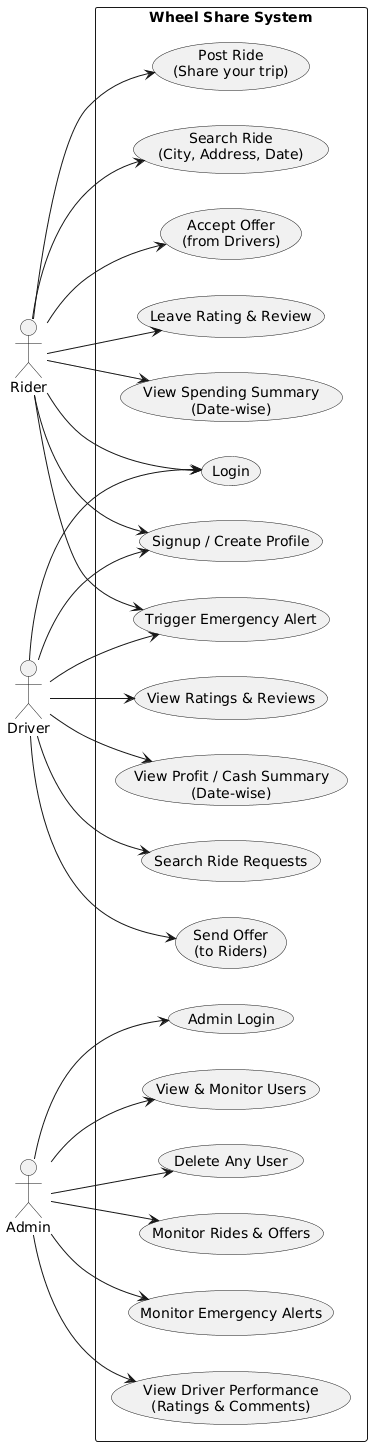
\includegraphics[height=0.95\textheight, keepaspectratio]{usecase_wheelshare.png}
    \caption{Use Case Diagram}
    \label{fig:usecase-diagram}
\end{figure}

\section{Use Case Specifications}


\subsection{Use Case: User Login}

\begin{table}[H]
\centering

\label{tab:usecase-login}
\renewcommand{\arraystretch}{1.2}
\begin{tabular}{|>{\bfseries}l|p{10cm}|}
\hline
Use Case ID & UC001 \\ \hline
Actor & User, Driver, Admin \\ \hline
Trigger & User submits credentials. \\ \hline
Pre-Condition & Registered user account exists. \\ \hline
Post-Condition & User successfully authenticated. \\ \hline
Flow &
1. User opens the app. \newline
2. User selects the login option. \newline
3. User enters login details. \newline
4. System verifies the account. \newline
5. User completes the login process. \\ \hline
\end{tabular}
\caption{Use Case for User Login}
\end{table}

\noindent
\textbf{Description:} This use case describes the authentication process where users log in using valid credentials and are redirected to their respective dashboards.

\subsection{Use Case: Sign Up}

\begin{table}[H]
\centering

\label{tab:usecase-signup}
\renewcommand{\arraystretch}{1.2}
\begin{tabular}{|>{\bfseries}l|p{10cm}|}
\hline
Use Case ID & UC002 \\ \hline
Actor & Rider, Driver \\ \hline
Trigger & User opens the sign-up page. \\ \hline
Pre-Condition & Email is not already registered. \\ \hline
Post-Condition & Account is created and profile is saved. \\ \hline
Flow &
1. User enters personal details. \newline
2. User verifies email. \newline
3. User creates profile. \newline
4. User logs into the system. \\ \hline
\end{tabular}
\caption{Use Case for Sign Up}
\end{table}

\noindent
\textbf{Description:} This use case explains the registration process for new users to create an account and access the system.


\subsection{Use Case: Post Ride}

\begin{table}[H]
\centering

\label{tab:usecase-postride}
\renewcommand{\arraystretch}{1.2}
\begin{tabular}{|>{\bfseries}l|p{10cm}|}
\hline
Use Case ID & UC003 \\ \hline
Actor & Rider \\ \hline
Pre-Condition & Rider is logged into the system. \\ \hline
Post-Condition & Ride is stored and visible to drivers. \\ \hline
Flow &
1. Rider enters ride details. \newline
2. Rider submits the ride. \newline
3. Ride becomes available for joining. \\ \hline
\end{tabular}
\caption{Use Case for Post Ride}
\end{table}

\noindent
\textbf{Description:} This use case allows riders to post ride details so that drivers can view and join the ride.

\subsection{Use Case: Search Ride / Send Offer / Accept Offer}

\begin{table}[H]
\centering

\label{tab:usecase-ridesearch}
\renewcommand{\arraystretch}{1.2}
\begin{tabular}{|>{\bfseries}l|p{10cm}|}
\hline
Use Case ID & UC004 \\ \hline
Actors & Rider, Driver \\ \hline
Pre-Condition & User is logged in and rides are available. \\ \hline
Post-Condition & Ride is confirmed if offer is accepted. \\ \hline
Flow &
1. Driver searches available rides. \newline
2. Driver sends an offer. \newline
3. Rider accepts or rejects the offer. \\ \hline
\end{tabular}
\caption{Use Case for Ride Search and Offer Management}
\end{table}

\noindent
\textbf{Description:} This use case defines the interaction between riders and drivers for ride matching and confirmation.




\subsection{Use Case: Ratings and Reviews}

\begin{table}[H]
\centering

\label{tab:usecase-ratings}
\renewcommand{\arraystretch}{1.2}
\begin{tabular}{|>{\bfseries}l|p{10cm}|}
\hline
Use Case ID & UC005 \\ \hline
Actors & Rider, Driver \\ \hline
Trigger & Completion of a ride. \\ \hline
Pre-Condition & Ride must be completed successfully. \\ \hline
Post-Condition & Feedback is saved and displayed. \\ \hline
Flow &
1. User selects completed ride. \newline
2. User submits rating and review. \\ \hline
\end{tabular}
\caption{Use Case for Ratings and Reviews}
\end{table}

\noindent
\textbf{Description:} This use case allows users to rate each other and provide feedback after a completed ride.


\subsection{Use Case: Spending Summary}

\begin{table}[H]
\centering

\label{tab:usecase-summary}
\renewcommand{\arraystretch}{1.2}
\begin{tabular}{|>{\bfseries}l|p{10cm}|}
\hline
Use Case ID & UC006 \\ \hline
Actors & Rider, Driver \\ \hline
Trigger & User opens summary module. \\ \hline
Pre-Condition & Ride history exists. \\ \hline
Post-Condition & Summary is displayed. \\ \hline
Flow &
1. User selects date range. \newline
2. System displays earnings or spending. \\ \hline
\end{tabular}
\caption{Use Case for Spending Summary}
\end{table}

\noindent
\textbf{Description:} This use case enables users to track their earnings or spending within a selected time period.

\subsection{Use Case: Emergency Feature}

\begin{table}[H]
\centering

\label{tab:usecase-emergency}
\renewcommand{\arraystretch}{1.2}
\begin{tabular}{|>{\bfseries}l|p{10cm}|}
\hline
Use Case ID & UC007 \\ \hline
Actors & Rider, Driver, Admin \\ \hline
Trigger & User presses emergency button. \\ \hline
Pre-Condition & Ride is ongoing. \\ \hline
Post-Condition & Emergency alert is logged. \\ \hline
Flow &
1. User triggers alert. \newline
2. System notifies admin. \\ \hline
\end{tabular}
\caption{Use Case for Emergency Feature}
\end{table}

\noindent
\textbf{Description:} This use case ensures user safety by allowing emergency alerts during an active ride.


\subsection{Use Case: Admin Monitoring}

\begin{table}[H]
\centering

\label{tab:usecase-admin}
\renewcommand{\arraystretch}{1.2}
\begin{tabular}{|>{\bfseries}l|p{10cm}|}
\hline
Use Case ID & UC008 \\ \hline
Actors & Admin \\ \hline
Trigger & Admin logs into the system. \\ \hline
Pre-Condition & Admin authentication successful. \\ \hline
Post-Condition & System activities are monitored. \\ \hline
Flow &
1. Admin monitors users and rides. \newline
2. Admin manages emergency alerts. \\ \hline
\end{tabular}
\caption{Use Case for Admin Monitoring}
\end{table}

\noindent
\textbf{Description:} This use case allows the administrator to monitor system activities and manage users.


\section{Project Feasibility}
The Wheel Share solution is most likely to be realized since it is based on open source technologies that prove to be inexpensive and have a scalable architecture. Flutter and Supabase can be used to dramatically decrease development cost and provide high-performing and cross-platform compatibility. The modularity of the application helps to make the future development of the app easier and manageable in terms of maintenance. Its friendly interface, which is based on the secure backend management, makes it applicable in the real world application. Besides, it covers the issues of affordability, convenience and safety thus finding its place in the area of community ride-sharing which makes the system sustainable in terms of urban mobility. 



\chapter{Design}
The architecture of the Wheel Share system is intended at developing scalable, secure, user-friendly ride sharing service that may be used by multiple users Rider, Driver, and Admin to serve in each of the mobile and web environments. The chapter gives a summary of the architectural structure, design limitations, and approach to be used in order to provide an unhindered user experience, performance of the system, and flexibility to experience future expansion. Since Wheel Share incorporates real-time data processing and cloud-based systems, it was stressed that proper planning and modular design were necessary to ensure that the system was efficient, had a high level of maintainability, and reliability of all the components\cite{mitropoulos2021}.


\section{System Architecture}
Wheel Share system is based on a service-oriented architecture that is modular to guarantee flexibility and scalability. It uses Flutter to develop cross-platform front-end forms, which could serve both mobile and web consumers. The client connects to Supabase services Authentication, PostgreSQL Database, and Storage, and Realtime channels via secure HTTP connections via JWT-modified sessions. 
The PostgreSQL uses Row-Level Security (RLS) policies to provide Role-Based Access Control (RBAC) to guarantee that users can only retrieve data that they are allowed to access by their role.  

A database has information that is important (user profiles, ride details, offers, emergency alerts, and so on) whereas Supabase storage has media files such as ride pictures or payment receipts. The use of this architecture provides secure communication, reliable data storage and real time synchronization of rides, offers and emergency notifications throughout the platform\cite{taiebat2022}.

\begin{figure}[H]
    \centering
    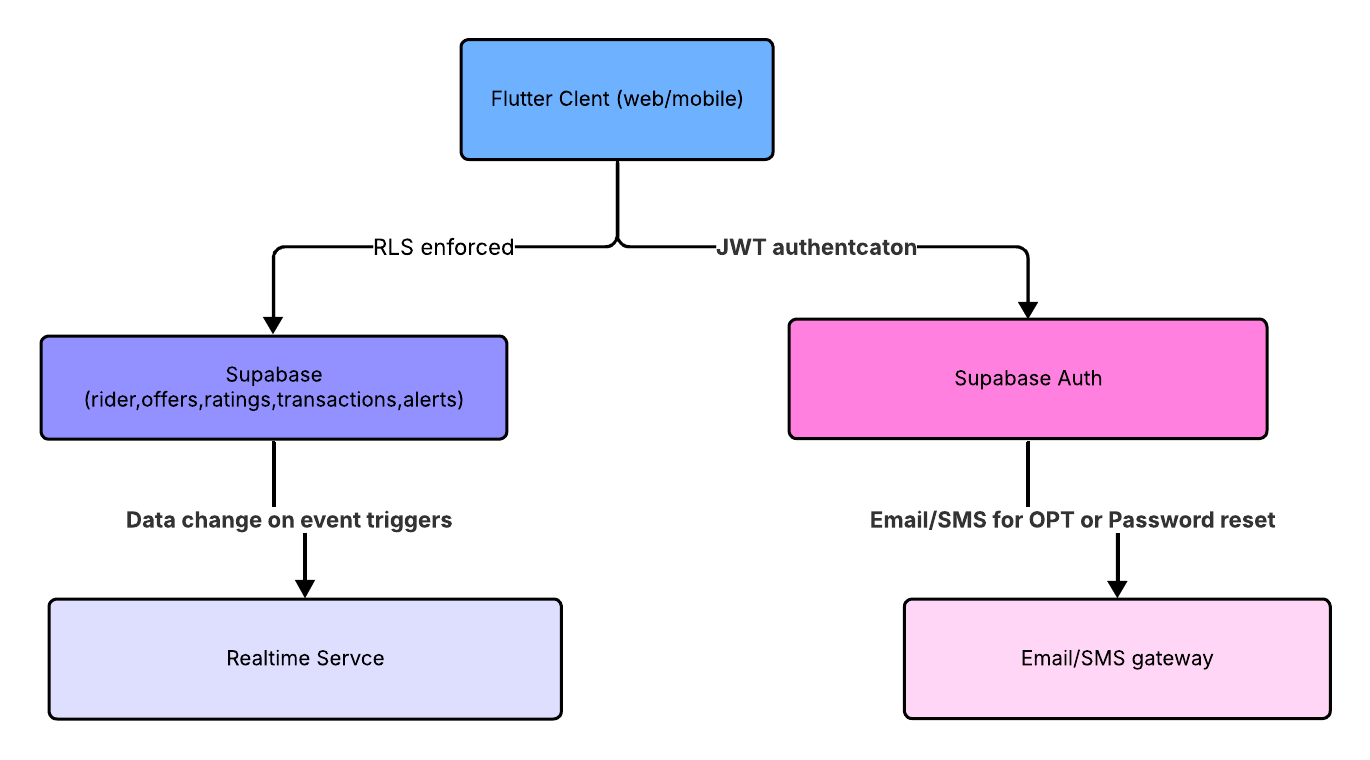
\includegraphics[width=0.9\textwidth,height=0.5\textheight]{Thought web weaver.png} 
    \caption{System Architecture Design}
    \label{fig:system-architechture-diagram}
\end{figure}
\noindent
\textbf{Description:} This architecture illustrates the interaction between the Flutter client, Supabase backend, and authentication services. The Flutter web/mobile client communicates with Supabase using JWT-based authentication, where Row Level Security (RLS) ensures controlled data access. Supabase Auth manages user authentication and handles email based OTP and password reset through an external gateway. Any data changes in the Supabase database trigger real-time services, enabling instant updates for rides, offers, ratings, transactions, and emergency alerts within the system.



\section{Design Constraints}
When designing Wheel Share, there were a number of technical, environmental, and operational factors that were used to design the system in a manner that satisfies its operation in the real-life state. 

\begin{itemize}
    \item \textbf{Software Requirements:} The browser Wheel Share should be compatible with latest software like Google Chrome or Microsoft Edge or Android mobile platforms. The communication with Supabase services through HTTPS requires a stable internet connection. Moreover, authentication and password recovery messages will also need an organization email account. 
    \item \textbf{Development Environment Requirements:} The programming languages needed in the front-end development are Flutter SDK (greater than 3.x) and Dart programming language. IDEs: the IDEs may be VS Code or Android Studio. It can be run with the aid of the backend using Supabase, and formatted with the help of SQL migration tools with the help of web-based Supabase Dashboard
    \item \textbf{Frameworks and Programming Language:} The front-end Flutter Dart of the system is reactive and has the successful state management. It also has a Supabase-based backend which contains PostgreSQL and structured data storage, Authentication and secure user management, storage and media management, and real-time updates. In addition, emergency alerts and receive notifications both will be the secure workflows that will be implemented on serverless Edge Functions. 
     \item \textbf{Technical Limitations:} Storage space and network latency of mobile browsers are also restricted by limitations of system performance, therefore, can have an impact on real-time ride updates and notifications. Besides, real time capabilities scalability depends on Supabase project which are the number of concurrent WebSocket connections and the number of concurrent requests.
     \item \textbf{Assumptions:} I believe the user familiar with the cardinal ride-sharing is involved in the activities of posting rides, making and accepting offers and rating rides. The fact that the drivers are supposed to be aware of the availability of the rides also questions them assuming that the emergency alerts will be monitored by the administrators at any given time. 

\end{itemize}

\section{Design Methodology}
The Wheel Share development and design process is modular and structure based which is premised on an \textbf{Agile development methodology}. The system is divided into logical modules that are easy to understand and they can be maintained at the same time as they can be developed.
\begin{itemize}
    \item \textbf{Partitioning: } The system is separated by features into Rider, Driver, and Admin modules and has some common services like Authentication, Ride Management, and Notifications. The database is partitioned to use separate tables that contain the data of the Users, Rides, Offers, Ratings, Transactions, and Emergency Alerts. Time based partitioning is used to manage asynchronous jobs such as the summary of earnings or expenditure and the delivery of timely notifications. 
    \item \textbf{Communication Requirements:} Communication between the client and Supabase is fully complete via the HTTPS protocol using tokens through in the authorization header. Instant synchronization, e.g. new offers, ride confirmations and emergency alerts are handled through WebSocket channels. 
    \item \textbf{Agglomeration Strategy:} Shared ride-list, offer management and rating display UI widgets are used to achieve design efficiency and re-usability of code. Database views are developed to make complex queries easier. 
    \item \textbf{Mapping:} Flutter has route guards that are mapped to role based permissions to ensure that only Riders, Drivers and admin can gain access of an authorized section. Database entities like Rides and Offers are implemented with RLS policies, and Edge Functions are implemented to automatically notify the administrator and emergency contacts in case an alert is fired. 

\end{itemize}

\begin{figure}[H]
    \centering
    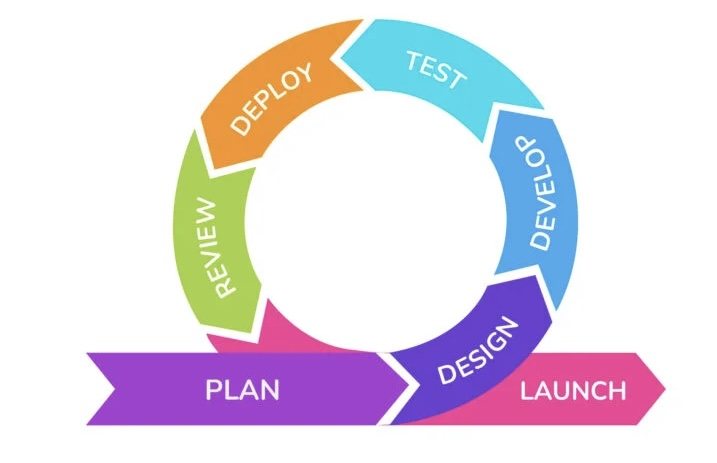
\includegraphics[width=0.6\textwidth]{agile.jpg} 
    \caption{Agile Methodology}
    \label{fig:agile-methodology-diagram}
\end{figure}

\section{High-Level Design}

The high level design of Wheel Share names the key elements of the system and their interaction process to attain the desired functionality. It focuses primarily on the database design and entity relationships, which guarantee efficient storage, retrieval and connectivity of the information of the user and the ride. 

\begin{itemize}
 \item \textbf{User:} Keeps information about customers like user-Id, name, email, role- Rider/Driver and profile description. 
 \item \textbf{Ride:} Ride data are stored in the stores and include ride related data such as source, destination, city, address, date and rider identification. 
 \item \textbf{Provide:} Relates rides/drivers and offers four fields of offer-Id, ride-Id, driver-Id and offer-Status.
 \item \textbf{Rating:} : It is used in rating the rides and is contained of rating-Id, ride-Id, reviewer-Id, score, and comments. 
 \item \textbf{Transaction:} : This table records all the transactions by transaction-Id, ride-Id, user-Id, amount and type (earning/ spending). 
 \item \textbf{Emergency Alert:} : Responsible of handling alerts like alert-Id,ride-Id,timestamp and status. 
\end{itemize}
\clearpage

\subsection{User Login Authentication and Authorization Flow}


\begin{figure}[H]
    \centering
    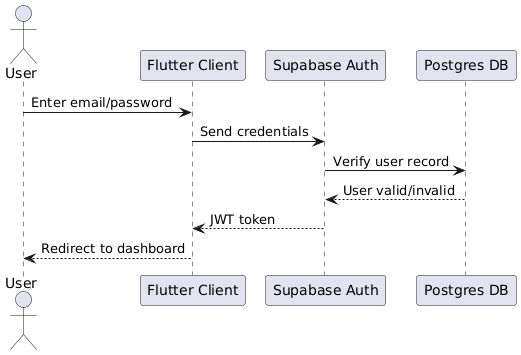
\includegraphics[width=1.0\textwidth]{HLD 1.png}
    \caption{User Login Sequence Diagram Using Flutter and Supabase Authentication}
    \label{fig:Sequence-diagram}
\end{figure}

\noindent
\textbf{Description:} This sequence diagram shows the user login process in the system. The user enters credentials through the Flutter client, which are sent to Supabase Authentication for verification. Supabase Auth validates the user using the PostgreSQL database. After successful authentication, a JWT token is generated and the user is redirected to the dashboard.
\clearpage


\subsection{Ride Posting and Real-Time Notification Flow}


\begin{figure}[H]
    \centering
    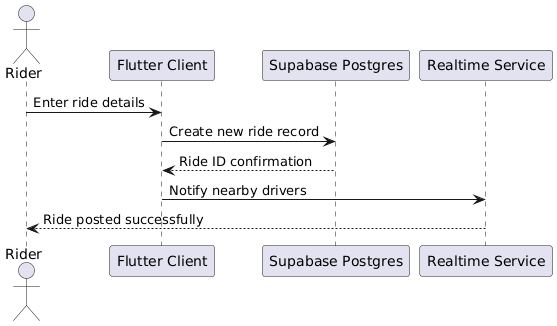
\includegraphics[width=1.0\textwidth]{HLD 2.png}
    \caption{Ride Posting Sequence Diagram}
    \label{fig:ride-posting-sequence}
\end{figure}

\noindent
\textbf{Description:} This sequence diagram illustrates the ride posting process performed by a rider. The rider enters ride details through the Flutter client, which creates a new ride record in the Supabase PostgreSQL database. Once the ride is successfully stored, a ride ID is generated. The real-time service then notifies nearby drivers about the newly posted ride.
\clearpage



\subsection{Offer Management and Ride Confirmation Flow}


\begin{figure}[H]
    \centering
    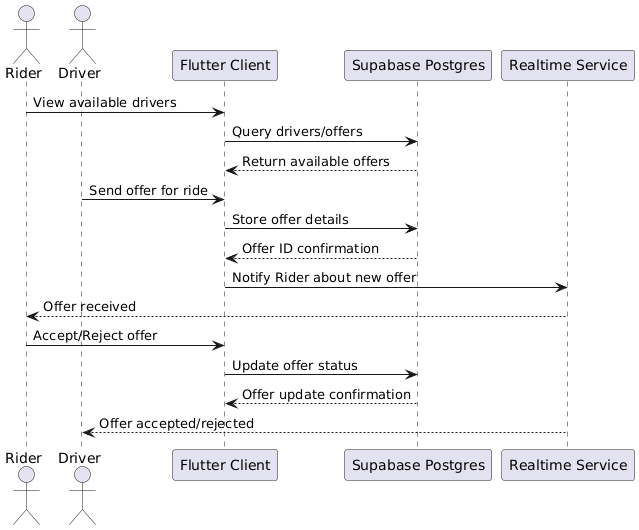
\includegraphics[width=1.0\textwidth]{HLD 3.png}
    \caption{Offer Management Sequence Diagram}
    \label{fig:offer-management-sequence}
\end{figure}

\noindent
\textbf{Description:} This sequence diagram shows the offer management process between riders and drivers. Drivers view available rides and send offers through the Flutter client, which are stored in the Supabase PostgreSQL database. The real-time service notifies riders about new offers. Riders can accept or reject offers, and the system updates the offer status accordingly.
\clearpage


\subsection{Emergency Alert Handling and Notification Flow}


\begin{figure}[H]
    \centering
    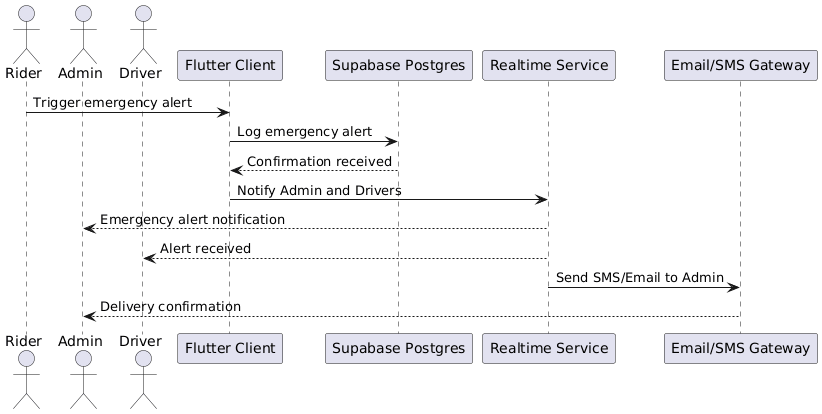
\includegraphics[width=1.0\textwidth]{HLD 4.png}
    \caption{Emergency Alert Handling Sequence Diagram}
    \label{fig:emergency-alert-sequence}
\end{figure}

\noindent
\textbf{Description:} This sequence diagram illustrates how emergency alerts are handled within the system. When a rider triggers an emergency alert, the Flutter client logs the alert in the Supabase PostgreSQL database. The real-time service notifies the admin and drivers instantly, while the Email/SMS gateway sends notifications to ensure timely response and user safety.



\section{Low-Level Design}

Each system component's specific structure is specified in the WheelShare Low-Level Design. With distinct interfaces and internal logic, it divides the program into smaller parts, including ride posting, ride search, offer handling, emergency alarms, admin monitoring, and authentication. In addition to offering a clear implementation plan, this modular approach guarantees that the code is simple to create, maintain, and reuse.
\clearpage
\subsection{Post Ride Submission and Validation Workflow}


\begin{figure}[H]
    \centering
    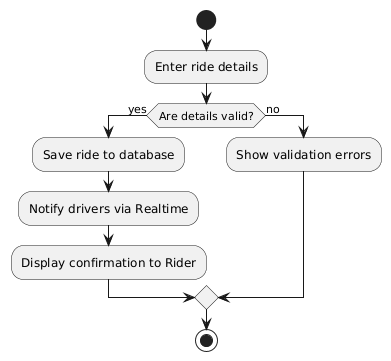
\includegraphics[width=1.0\textwidth]{LLD 1.png} 
    \caption{Post Ride Process Activity Diagram}
    \label{fig:post-ride-activity}
\end{figure}

\noindent
\textbf{Description:} This activity diagram represents the workflow of posting a ride in the system. The rider enters ride details, which are first validated by the system. If the details are valid, the ride is saved to the database and nearby drivers are notified through the real-time service; otherwise, validation errors are displayed to the rider.

\clearpage
\subsection{Ride Offer Acceptance and Rejection Workflow}


\begin{figure}[H]
    \centering
    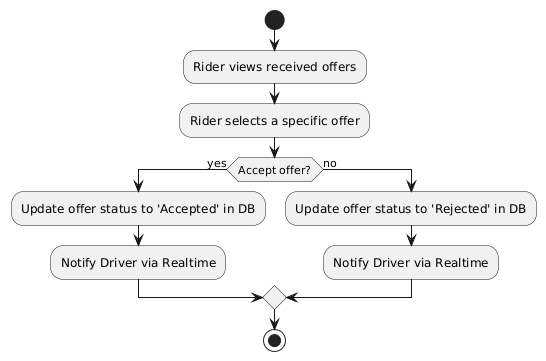
\includegraphics[width=1.0\textwidth]{LLD 2.png} 
    \caption{Accept Offer Process Activity Diagram}
    \label{fig:accept-offer-activity}
\end{figure}

\noindent
\textbf{Description:} This activity diagram illustrates the process of handling ride offers by the rider. The rider views received offers and selects a specific offer to accept or reject. Based on the decision, the system updates the offer status in the database and notifies the driver in real time.





\section{GUI Design}
Wheel Share is built with Flutter as its Graphical User Interface (GUI) to provide a similar and dynamic experience in the mobile and web interfaces. The interface is centered upon the clarity, access and ease of navigation. A bottom navigation bar or a layout based on tabs enables the users to have a quick reach to the basic functions such as posting rides, looking at offers, checking the earnings or spending, and causing emergency notifications. It is minimalistic and easy to use in design: there are no icons or labels, the color schemes are balance-oriented, and the input forms fit on a mobile screen. The system can also incorporate real-time notification of offers, confirmation and alerting to ensure continuous information to the users.  

\section{Mobile App Interface}

The Flutter-based GUI was developed with a focus on:


\subsection{Initial App Launch and Location Permission Screen}


\begin{figure}[H]
    \centering
    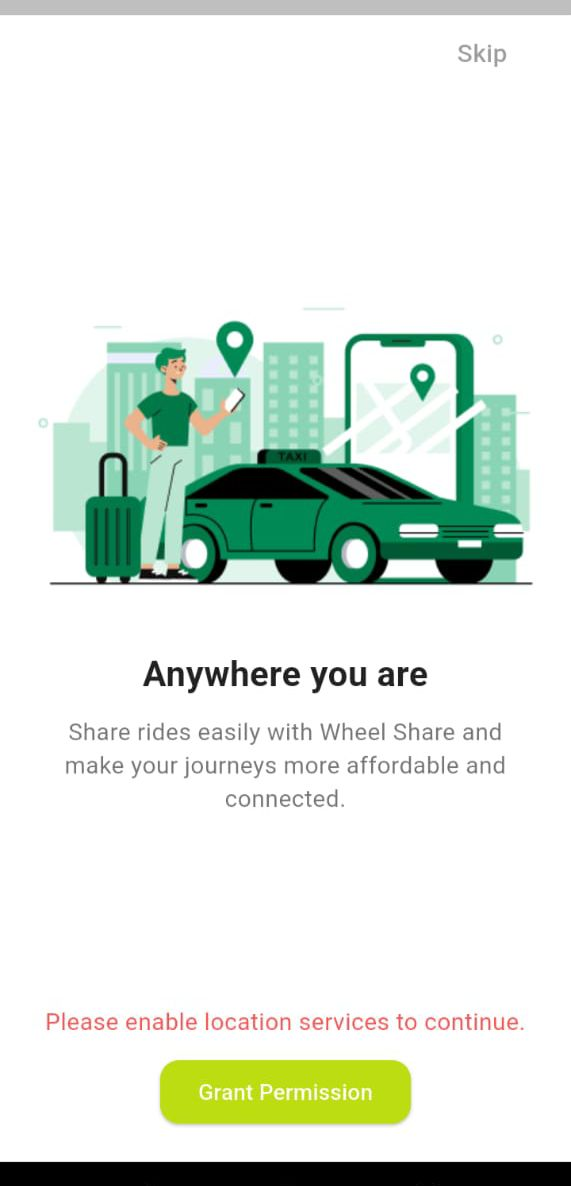
\includegraphics[width=0.6\textwidth,height=16cm]{frontt.jpeg} 
    \caption{Initial screen displayed when the application is installed}
    \label{fig:initial-app-screen}
\end{figure}

\noindent
\textbf{Description:} This screen is displayed when the application is launched for the first time after installation. It requests location permission to enable nearby ride discovery and navigation features.
\clearpage


\subsection{User Registration (Sign Up) Interface}


\begin{figure}[H]
    \centering
    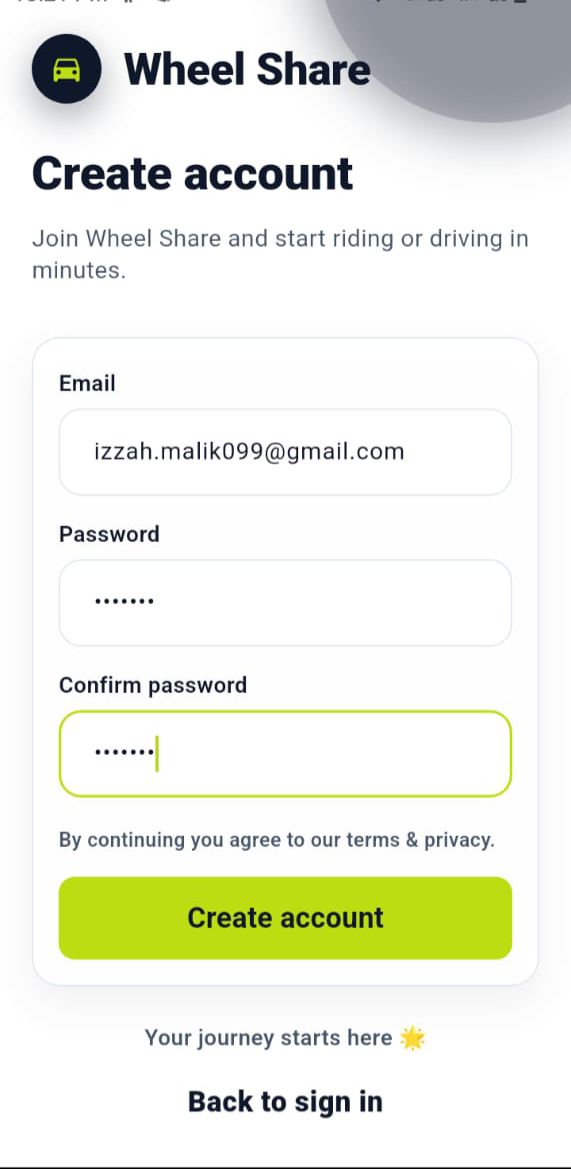
\includegraphics[width=0.6\textwidth,height=17.5cm]{sign.jpeg} 
    \caption{Sign Up Page}
    \label{fig:signup-gui}
\end{figure}

\noindent
\textbf{Description:} This interface enables new users to register by providing their email and password information. Upon successful registration, users gain access to the core functionalities of the application.
\clearpage


\subsection{ Admin Dashboard and System Monitoring Interface}


\begin{figure}[H]
    \centering
    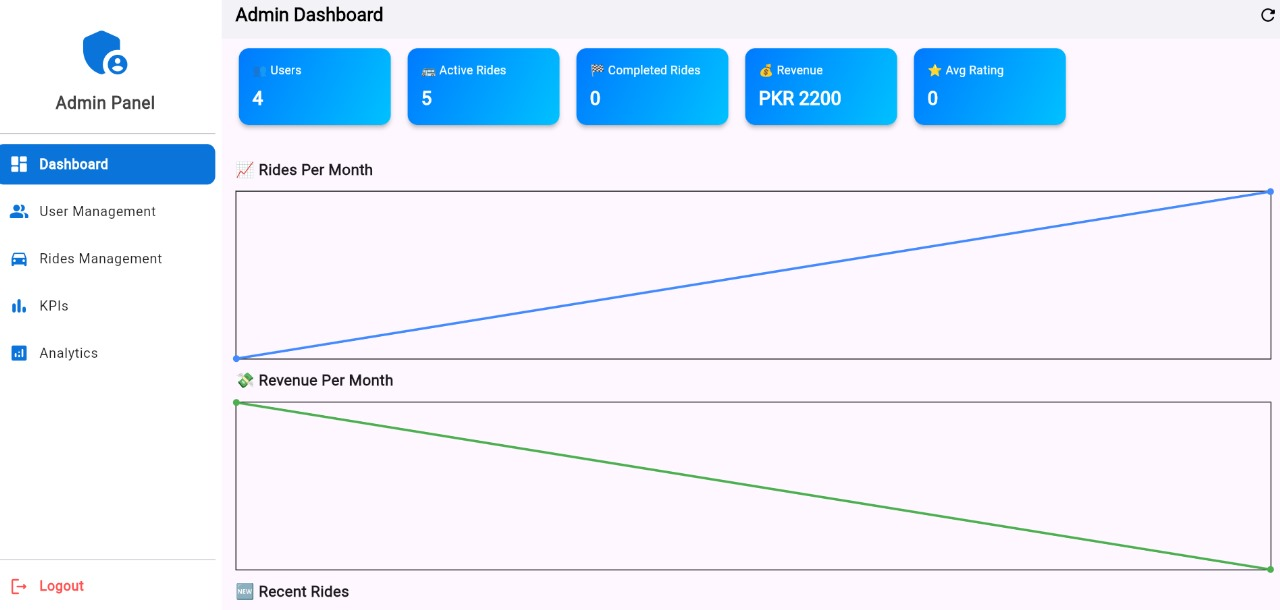
\includegraphics[width=0.9\textwidth,height=16cm]{WhatsApp Image 2025-11-24 at 6.47.08 PM.jpeg}
    \caption{Admin Page}
    \label{fig:admin-gui}
\end{figure}

\noindent
\textbf{Description:} This dashboard allows the admin to monitor system activity, including users, rides, and revenue statistics. It also provides analytical insights through graphs to support system management and decision-making.
\clearpage


\subsection{User Authentication (Login) Interface}


\begin{figure}[H]
    \centering
    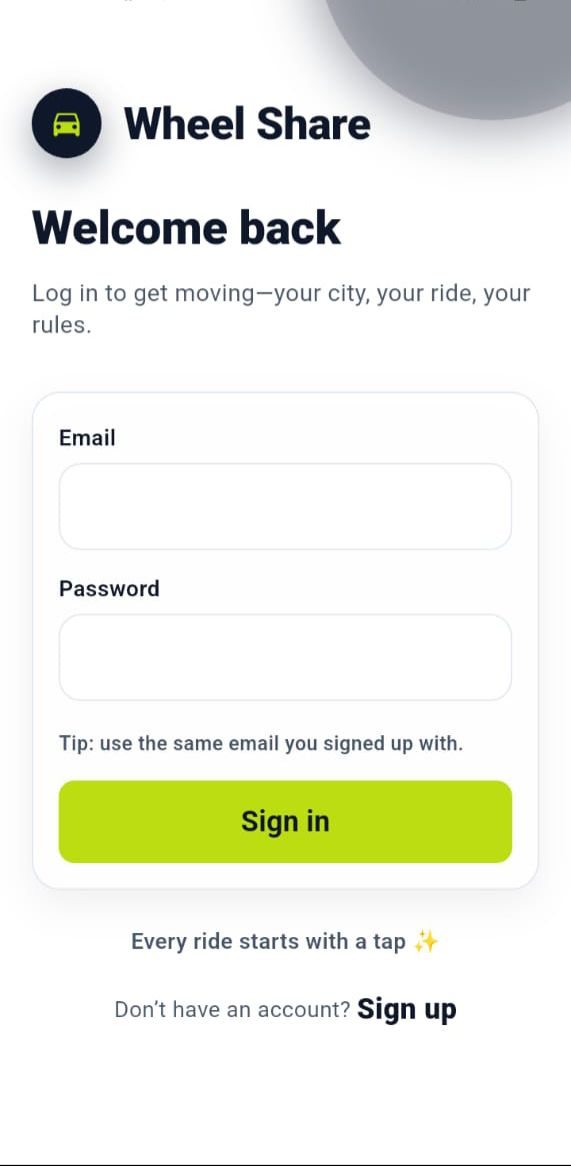
\includegraphics[width=0.6\textwidth,height=17.5cm]{loginp.jpeg} 
    \caption{Login Page}
    \label{fig:login-gui}
\end{figure}

\noindent
\textbf{Description:} This screen allows registered users to log in by entering their email and password credentials. Successful authentication grants access to personalized dashboards and ride-sharing features.
\clearpage



\subsection{User Profile and Account Information Interface}


\begin{figure}[H]
    \centering
    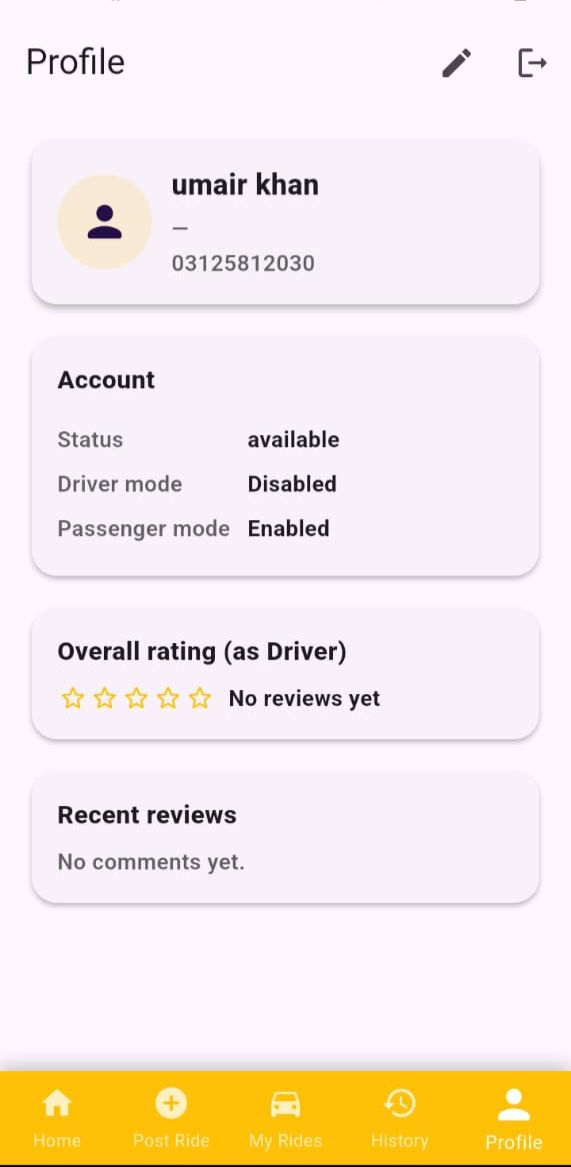
\includegraphics[width=0.6\textwidth,height=17.5cm]{user.jpeg} 
    \caption{User Profile}
    \label{fig:user-profile-gui}
\end{figure}

\noindent
\textbf{Description:} This screen displays the user’s personal details, account status, and role preferences. It also shows driver ratings and recent reviews to support trust and transparency within the system.
\clearpage


\subsection{Ride Posting Interface}


\begin{figure}[H]
    \centering
    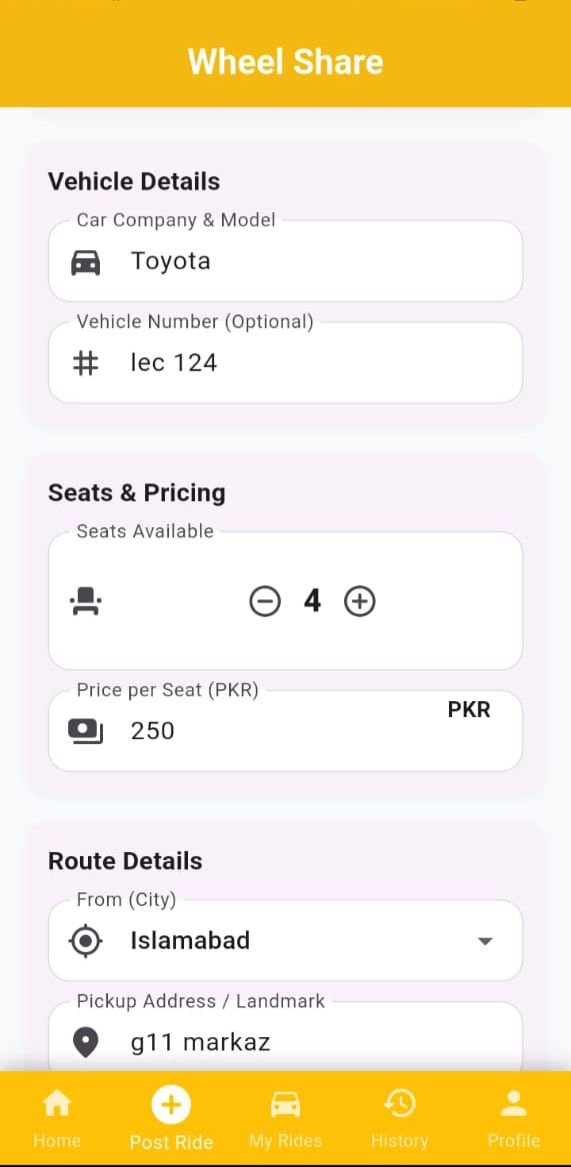
\includegraphics[width=0.6\textwidth,height=17.5cm]{ride posted.jpeg} 
    \caption{User Post Ride}
    \label{fig:post-ride-gui}
\end{figure}

\noindent
\textbf{Description:} This interface allows users to post a ride by entering vehicle, pricing, and route details. Once submitted, the ride becomes available for drivers or passengers to view and join.
\clearpage

\subsection{Location Selection for Ride Posting}


\begin{figure}[H]
    \centering
    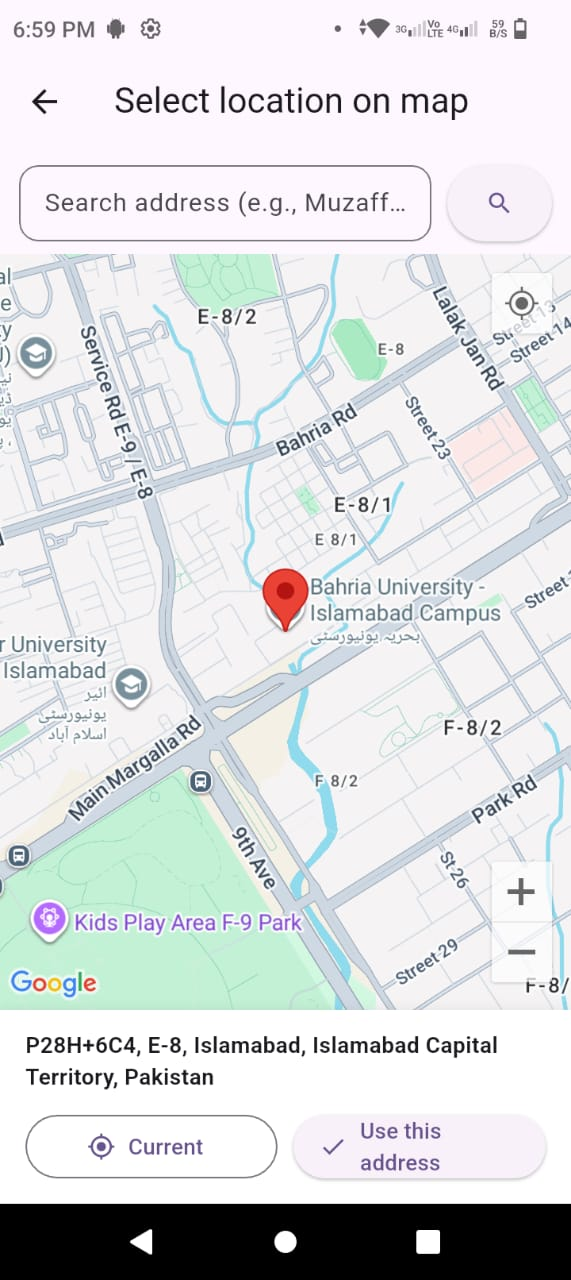
\includegraphics[width=0.6\textwidth,height=17.5cm]{WhatsApp Image 2025-12-14 at 7.00.35 PM.jpeg} 
    \caption{Map-Based Location Selection Screen}
    \label{fig:location-selection-gui}
\end{figure}

\noindent
\textbf{Description:} This screen allows users to select the pickup or destination location directly from the map. The selected address is used to ensure accurate routing and ride matching within the system.
\clearpage



\subsection{Ride Details and Availability Interface}


\begin{figure}[H]
    \centering
    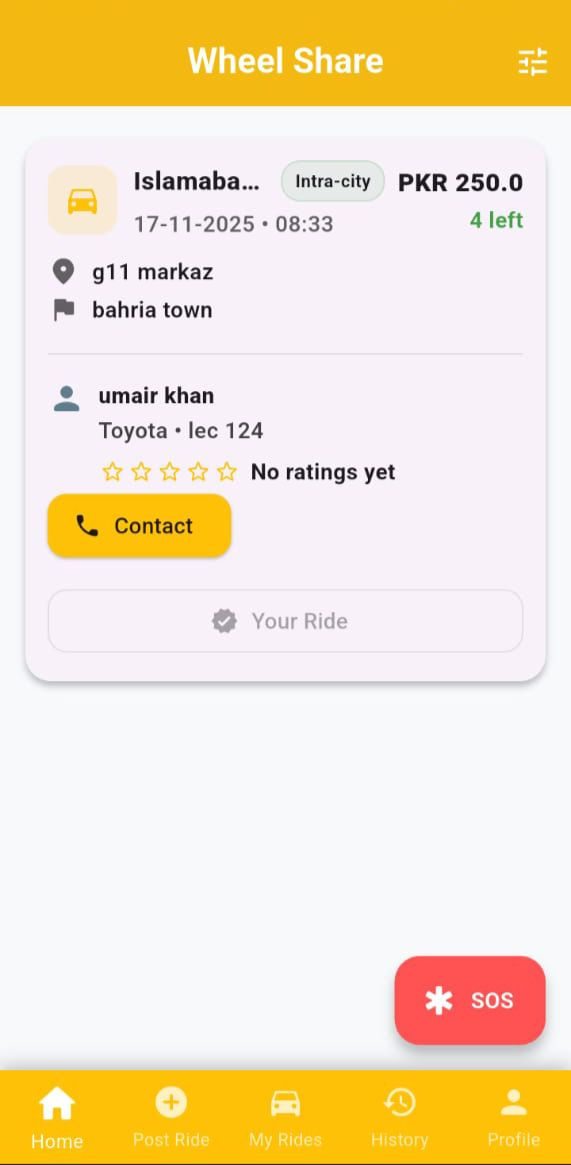
\includegraphics[width=0.6\textwidth,height=17.5cm]{avail.jpeg} 
    \caption{Ride Sharing Details}
    \label{fig:ride-details-gui}
\end{figure}

\noindent
\textbf{Description:} This screen displays detailed information about an available ride, including route, time, price, and driver details. Users can contact the driver or view ride status directly from this interface.
\clearpage


\subsection{Driver Ride Management Interface}


\begin{figure}[H]
    \centering
    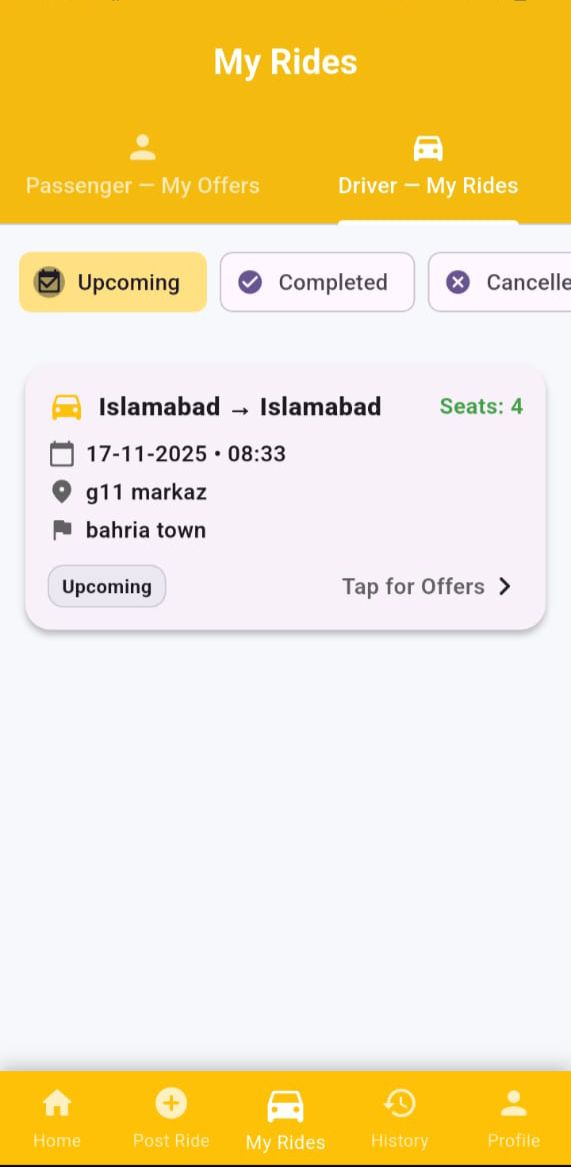
\includegraphics[width=0.6\textwidth,height=17.5cm]{dr ofer.jpeg} 
    \caption{Driver Offer a Ride}
    \label{fig:driver-offer-gui}
\end{figure}

\noindent
\textbf{Description:} This screen allows drivers to view and manage their posted rides, including upcoming and completed trips. Drivers can also review ride details and track available seats from this interface.
\clearpage


\subsection{Passenger Ride Offers Dashboard}


\begin{figure}[H]
    \centering
    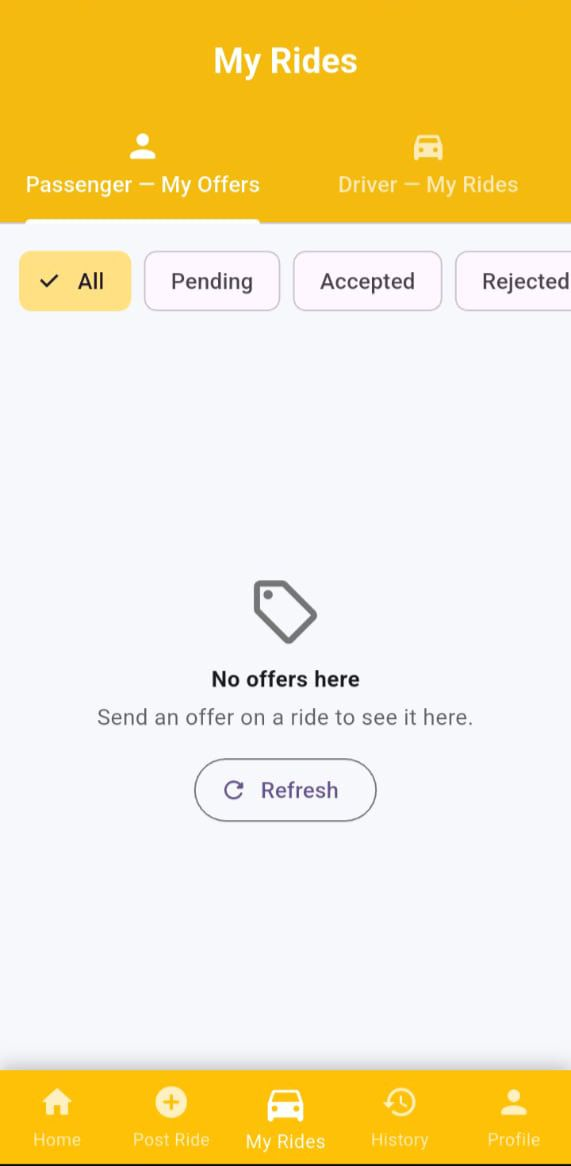
\includegraphics[width=0.6\textwidth,height=17.5cm]{psngr.jpeg} 
    \caption{Passenger Dashboard}
    \label{fig:passenger-dashboard-gui}
\end{figure}

\noindent
\textbf{Description:} This dashboard allows passengers to view and manage ride offers they have sent or received. Offers can be filtered by status such as pending, accepted, or rejected for easy tracking.
\clearpage

\subsection{History Dashboard}


\begin{figure}[H]
    \centering
    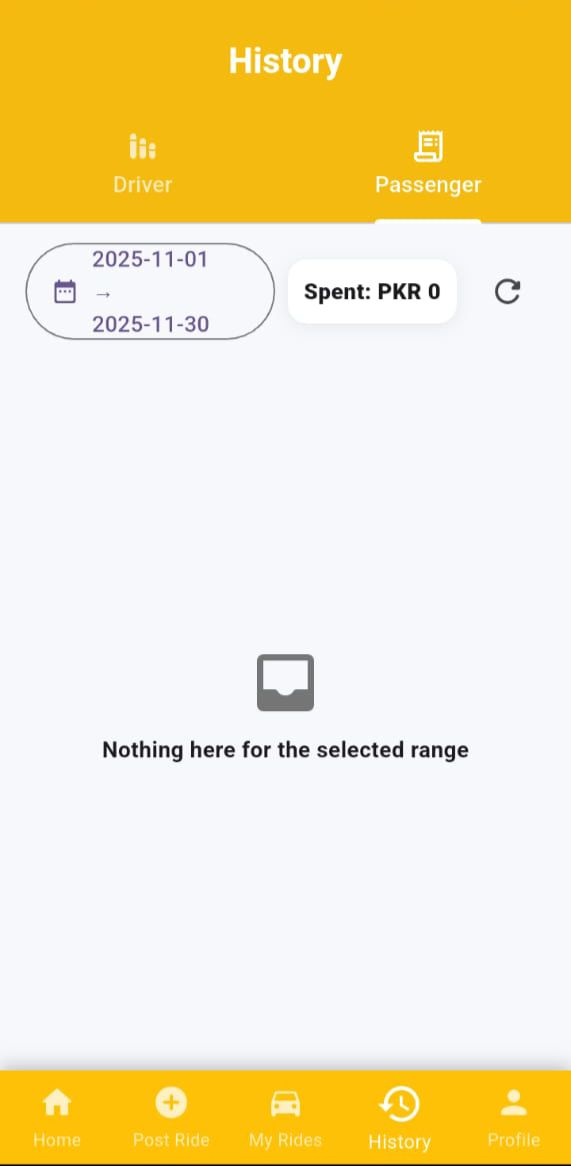
\includegraphics[width=0.6\textwidth,height=17.5cm]{his.jpeg}
    \caption{History Dashboard}
    \label{fig:history-dashboard-gui}
\end{figure}

\noindent
\textbf{Description:} This dashboard enables users to view their ride history within a selected date range and track total spending. If no rides exist for the chosen period, the system clearly indicates the absence of records.


\clearpage

\section{External Interfaces }
To provide a very efficient, safe and smooth experience Wheel Share works with various external services. Supabase is an authentication that provides user authentication, transactions, and passwords. Supabase database is a postgreSQL that handles operations related to ride, offers, transactions, and log emergency in addition to providing RLS as protection. 
The ride-related images, documents or receipts are stored securely by Supabase storage on signed URLs that provide limited access. The Realtime Service allows the use of the WebSocket channel on two-way communication to immediately update status, and the Email Gateways serve to notify about the offer acceptance, ride confirmations, and emergency messages. All external communication is carried out through the HTTPS or web socket protocols and the authentication is used to have secure and role-based access to data and integrity. 

 




\chapter{System Implementation}
The chapter explains the steps that the WheelShare system implementation process will follow, how the conceptual design may be transformed into a completely effective, intelligent carpooling service. It explains the development of the frontend, backend and database parts, their integration, and testing to address the nonfunctional and functional requirements. Its building system is based on Flutter and cross-platform mobile and web application but Supabase is the backend service, which supports authentication, storage, real-time updates, and database management. 

\section{System Architecture}
WheelShare architecture is a programmed system to be implemented as a modular and scalable system, whereby there is an efficient communication between components. It is applicable to visualization in form of three major layers:  
\begin{itemize}
    \item \textbf{Frontend (Flutter):} Its front is backed up by Flutter and provides role based dashboards to Riders, Drivers and Administrators. It enjoys simple structure; thus navigation and real-time updates of rides and responsive platforms of Android platforms, and Web platform can be easily navigated.

    \item \textbf{Backend Services (Supabase):} Its back-end is Supabase that is an engine and hosted by the following fundamental services: authentication, database management (PostgreSQL with Row-Level Security), file storage and realtime sync.  
 
    \item \textbf{Resource (Individual channels):} Live-time communication layer will deliver the live time information on the ride offers or confirmations, emergency notification and the state of the completion of the ride, which will give the user a perfect experience and data synchronization, in real-time. 
 
\end{itemize}

\section{Tools and Technologies}
The WheelShare solution is based on a new technology stack to provide efficiency, performance, and scalability. 

\begin{itemize}
    \item \textbf{Front-end Development:} Flutter (for Android, and Web) 
    \item \textbf{Backend Services:} Supabase (Auth, PostgreSQL, Storage, Realtime)
    
    \item \textbf{Database:} Secure unencrypted role-based data access in postgreSQL using Row-Level security (RLS). 
    \item \textbf{Programming Languages:} Dart (Frontend), SQL (Backend Policies 
    \item \textbf{IDE:} Visual Studio Code / Android Studio 
\end{itemize}
    

\section{Development Environment }
To ensure compatibility and stable performance, the following environment was used during development and testing: 

\begin{itemize}
    \item \textbf{Operating System:} Windows 11 
    \item \textbf{Testing Devices:} Android Emulator
    \item \textbf{SDKs:} Flutter 3.x, Dart 3.x 
    \item \textbf{Database:} Supabase PostgreSQL 15.x 
    \item \textbf{APIs:} Supabase REST endpoints and Realtime subscriptions 
    \item \textbf{Authentication:} Email and Password-based authentication via Supabase Auth  
    \end{itemize}
\section{Processing Logic / Algorithms}
The internal working of WheelShare follows several logical processes and algorithms that power its main features.

\subsection{Login and Role Routing}
\begin{enumerate}
    \item Validate user credentials via Supabase Auth.
    \item Retrieve user role from the Profiles table.
    \item Redirect the user to the corresponding dashboard Rider, Driver, or Admin.
\end{enumerate}

\subsection{Ride Posting and Offer Management}
\begin{enumerate}
    \item Rider creates a new ride post including source, destination, city, address, and date.
    \item Drivers can search available rides and send offers to Riders.
    \item Riders can accept or reject offers; once confirmed, rides are updated in the database.
    \item Realtime notifications are triggered upon any change in offer status.
\end{enumerate}

\subsection{Earnings and Spending Summary}
\begin{enumerate}
    \item Driver earnings and Rider spending are extracted from ride transaction records.
    \item Summaries are computed based on a selected date range.
    
\end{enumerate}

\subsection{Emergency Alert Handling}
\begin{enumerate}
    \item The user is able to activate an emergency alarm inside the app.
    \item The notification is immediately forwarded to Administrators and close registered contacts through Realtime notifications.
    \item All the alerts are documented in the database to be audited and analysed in future.
\end{enumerate}

\section{Integration with Supabase}
All the parts of the system interact with each other smoothly using the Flutter client SDK of Supabase. Supabase replaces a custom backend server and handles:

\begin{itemize}
    \item Authentication
    \item Database operations,File storage
    \item Realtime synchronization
\end{itemize}

\section{Testing and Deployment}
WheelShare system was thoroughly tested to ensure it is stable, secure and easy to use.

\subsection{Testing}
To guarantee system dependability, testing was done at several levels. Workflows for ride posting, offer acceptance, and authentication were all tested. Integration testing confirmed the accuracy of earnings and spending summaries as well as the processing of emergency alerts. UI testing concentrated on search filter efficacy, dashboard accessibility, and navigation. 

\subsection{Deployment}
Android platforms are used for mobile deployment. WheelShare's online version is hosted by Firebase Hosting or Supabase Hosting. GitHub Actions is used to manage Continuous Integration and Deployment (CI/CD), which guarantees automated builds, upgrades, and seamless delivery of new features.

\section{Security Measures}
WheelShare uses a number of security procedures to guarantee data safety. To ensure secrecy, sensitive data including login credentials is encrypted. While Row Level Security (RLS) stops unwanted access at the database layer, authentication and role-based access control limit users to the functions permitted for their roles. Additionally, the system keeps track of important activities like ride postings and warnings in real time for auditing purposes. Furthermore, secure HTTPS encrypted APIs are used for all connection between the app and Supabase to guarantee secure data transfer.





\chapter{System Testing and Evaluation}
In this chapter, the testing and evaluation process of the Wheel Share system will be introduced so that it should be effective and will address all the requirements of the user. Various forms of testing that include GUI testing, usability testing, performance testing, compatibility testing and exception handling were carried out in order to be assured that the system operates as desired by both the Riders, Drivers and Admins. 
\section{Importance of System Testing}
The tests on the system are critical to the quality and reliability of the Wheel Share application. It also checks that all the parts, such as posting of rides or accepting offers and emergency notifications, are functioning as desired. Systematic testing was also used to detect possible errors and rectify before real deployment. This would ensure that there is a user friendly and safe user experience and the system develops the confidence of the user in the performance and stability of the system\cite{chaudhry2018}.

\section{Graphical User Interface (GUI) Testing}
Graphical User Interface (GUI) testing will deal with confirming the visual and interactive interface of the Wheel Share app. All the screens and dashboards have been tested to launch menus, icons, buttons and flow of navigation both on the web and mobile platform. Responsiveness, consistency of layouts and accuracy of design were given special consideration. The interface was verified to be clean, intuitive and easy to use and offered a smooth navigation through the Riders, Drivers and Admins. 

\section{Usability Testing}
The usability testing was performed to determine the ease with which this application (Wheel Share) could be navigated and used by the users. A team of Riders, Drivers, and Admins were consulted to execute more routine duties including adding rides, taking in offers, and making emergency alerts. The findings revealed that the application was not only easy to navigate but was also user friendly with the instructions being very simple and very little process was involved to accomplish each task. The user-friendly design of the app enhanced the use experiences and satisfaction. 

\section{Software Performance Testing}
The performance testing was done to assess the behaviour of the Wheel Share system under different load directions. They tested the speed with which they could respond to the actions of ride search, offer submission and dashboard loading. The system did not have a decline in performance even upon having more users of the system simultaneously. The average search time of the ride took less than two seconds and the dashboard summary took an average of three seconds to load. These are the findings indicating the necessary requirements of scalability and speed of the application. 
\section{Compatibility Testing}
The compatibility testing was made to ensure that Wheel Share system will work across various devices, operating systems and browsers. The app has been made to work with Android, and web browsers, including Chrome, Edge, and Safari. It worked effectively in every platform it had similar graphic effects and functionality. This is to make sure that users can use Wheel Share in any modern gadget without any performance problems and disfiguration on the interface.
\section{Exception Handling}
Exception handling test was done to ensure that the system responds to the wrong or unexpected messages. The system showed relevant error messages when the users typed wrong credentials or left some required fields blank or even trying to do actions without authorization. This increased stability and avoided crashing of the systems so that all the users had a secure and stable environment. 

\section{Test Cases}
Various test cases were carried out to test the basic functionality of the system. These comprised of login authentication, Ride creation, offer management, emergency alert triggering, earnings and spending summaries. Every test case was verified to attest the proper functioning and system work. The system successfully passed the majority of test cases, having more than 95 percent accuracy on function test and integration test. 


\subsection{Test Case: Login}

\begin{table}[H]
\centering

\label{tab:testcase-login}
\renewcommand{\arraystretch}{1.2}
\begin{tabular}{|>{\bfseries}l|p{10cm}|}
\hline
Test Case ID & 0001 \\ \hline
Test Case & Login with valid credentials (Rider/Driver/Admin) \\ \hline
Pre-Conditions & User exists, email verified, active status \\ \hline
Steps &
1. Open login screen. \newline
2. Enter email and password. \newline
3. Submit the login form. \\ \hline
Expected Result & User is redirected to the respective dashboard and a secure session is established. \\ \hline
Actual Result & As expected \\ \hline
Status & Pass \\ \hline
\end{tabular}
\caption{Login Test Case}
\end{table}

\noindent
\textbf{Description:} This test case validates that authorized users can successfully log into the system using valid credentials and access their respective dashboards securely.




\subsection{Test Case: Ride Posting}

\begin{table}[H]
\centering
\label{tab:testcase-ride-post}
\renewcommand{\arraystretch}{1.2}
\begin{tabular}{|>{\bfseries}l|p{10cm}|}
\hline
Test Case ID & 0002 \\ \hline
Test Case & Rider: Post a Ride Request \\ \hline
Pre-Conditions & Rider logged in; ride form available \\ \hline
Steps &
1. Enter ride details (source, destination, date, time). \newline
2. Submit the ride request. \\ \hline
Expected Result & Ride request is saved successfully, becomes visible to drivers in the same city, and a notification is sent. \\ \hline
Actual Result & As expected \\ \hline
Status & Pass \\ \hline
\end{tabular}
\caption{Test Case for Ride Posting}
\end{table}

\noindent
\textbf{Description:} This test case verifies that a rider can successfully post a ride request and that the request is properly stored, displayed to relevant drivers, and notifications are triggered.


\subsection{Test Case: Driver Ride Offer}

\begin{table}[H]
\centering

\label{tab:testcase-driver-offer}
\renewcommand{\arraystretch}{1.2}
\begin{tabular}{|>{\bfseries}l|p{10cm}|}
\hline
Test Case ID & 0003 \\ \hline
Test Case & Driver: Offer Ride \\ \hline
Pre-Conditions & Driver logged in; rides available \\ \hline
Steps &
1. Select a ride post. \newline
2. Send ride offer. \newline
3. Rider accepts or rejects the offer. \\ \hline
Expected Result & Offer status is updated, real-time notifications are sent, and the ride is confirmed upon acceptance. \\ \hline
Actual Result & As expected \\ \hline
Status & Pass \\ \hline
\end{tabular}
\caption{Driver Ride Offer and Acceptance}
\end{table}

\noindent
\textbf{Description:} This test case ensures that drivers can successfully offer rides to riders and that the system correctly handles offer status updates, notifications, and ride confirmation.


\subsection{Test Case: Emergency Alert}

\begin{table}[H]
\centering

\label{tab:testcase-emergency-alert}
\renewcommand{\arraystretch}{1.2}
\begin{tabular}{|>{\bfseries}l|p{10cm}|}
\hline
Test Case ID & 0004 \\ \hline
Test Case & Emergency Alert Trigger \\ \hline
Pre-Conditions & User logged in; network connected \\ \hline
Steps &
1. Tap the emergency alert button. \newline
2. Confirm the emergency alert. \\ \hline
Expected Result & Notification is sent to the admin and emergency contacts, and the alert is logged in the database. \\ \hline
Actual Result & As expected \\ \hline
Status & Pass \\ \hline
\end{tabular}
\caption{Test Case for Emergency Alert Trigger}
\end{table}

\noindent
\textbf{Description:} This test case verifies that users can successfully trigger an emergency alert and that the system promptly notifies relevant authorities and records the alert for safety purposes.


\subsection{Test Case: Admin Dashboard}

\begin{table}[H]
\centering
\label{tab:testcase-admin-dashboard}
\renewcommand{\arraystretch}{1.2}
\begin{tabular}{|>{\bfseries}l|p{10cm}|}
\hline
Test Case ID & 0005 \\ \hline
Test Case & Admin: View Dashboard \& Ride Statistics \\ \hline
Pre-Conditions & Admin logged in; rides and users seeded \\ \hline
Steps &
1. Load the admin dashboard. \newline
2. Apply filters by city or date. \newline
3. Drill down into ride details. \\ \hline
Expected Result & Dashboard aggregates match the database records, and drill-down views display correct ride information. \\ \hline
Actual Result & As expected \\ \hline
Status & Pass \\ \hline
\end{tabular}
\caption{Test Case for Admin Dashboard and Ride Statistics}
\end{table}

\noindent
\textbf{Description:} This test case ensures that the admin can view accurate dashboard analytics and ride statistics, apply filters, and access detailed ride information correctly.


\subsection{Security Test Scenario}

\begin{table}[H]
\centering
\label{tab:testcase-security}
\renewcommand{\arraystretch}{1.2}
\begin{tabular}{|>{\bfseries}p{6cm}|p{8cm}|}
\hline
Test Scenario & Result / Enforcement \\ \hline
Unauthorized role attempts to accept rides on behalf of others & Action denied by role-level security (RLS) \\ \hline
Cross-city ride access attempt & No records returned due to access restrictions \\ \hline
Unsigned GET request to private profile images & Request blocked with 403 Forbidden response \\ \hline
SQL/JavaScript injection attempts via form inputs & No impact due to parameterized queries and input validation \\ \hline
Fake or modified emergency alert submission & Request denied by security policy enforcement \\ \hline
\end{tabular}
\caption{Negative and Security Test Results}
\end{table}

\noindent
\textbf{Description:} This security test scenario verifies that the system enforces role-based access control and protects against unauthorized access and common security vulnerabilities.





\chapter{Conclusion}
\section{Summary}
The Wheel Share has effectively provided a secure, scalable, user-friendly service to the citizens of the contemporary city, namely ride-sharing. The system is built to enable a modular structure and developed on Flutter to render cross-platform compatibility and Supabase as the backend service, which offers a single platform to the Riders, Drivers, and Administrators. It handles the necessity functionality like posting of rides, offering, real-time alerts, and emergency notifications\cite{mitropoulos2021}. 
There is also a seamless integration of Supabase to serve as an authentication tool, database management and real time communication tool to guarantee smooth data synchronization and security. 
In general, Wheel Share achieves its goals of establishing the safe, convenient, and efficient ride-sharing as well as building trust and reliability among consumers. The system creates a foundation on which scalable and data driven urban mobility solutions to accommodate future technological changes can fit through centralization of core operations into one framework. 

\section{Future Work}
To extend the performance and possibilities of the Wheel Share system, it can be seen that a number of improvements will be considered in its further development. Caching mechanisms, asynchronous query processing, and read replicas can be included in order to scalability and achieve good performance in order to maintain low-latency responses even when there is a high traffic. The application of AI-based automation may also enhance the precision of ride-matching, add dynamic fare suggestions, and also predictive notifications to foster more user interaction\cite{bujak2024}.

\clearpage


% ---------------- References ----------------
\clearpage
\renewcommand{\bibname}{References}
\addcontentsline{toc}{chapter}{References}

\begin{thebibliography}{99}

\bibitem{mitropoulos2021}
L. Mitropoulos, A. Kortsari, and G. Ayfantopoulou,
\textit{A systematic literature review of ride-sharing platforms, user factors and barriers},
European Transport Research Review, 13(61), 2021.

\bibitem{alonso2020}
M.J. Alonso-González et al.,
\textit{Determinants of willingness to share rides in ride-hailing},
PLoS ONE, 15(9), 2020.

\bibitem{gangadharaiah2023}
R. Gangadharaiah et al.,
\textit{Development of the pooled rideshare acceptance model (PRAM)},
Safety (MDPI), 9(3):61, 2023.

\bibitem{ashkrof2022}
P. Ashkrof et al.,
\textit{Ride acceptance behaviour of ride-sourcing drivers},
Transportation Research Part A: Policy and Practice, 160:182–197, 2022.

\bibitem{merat2017}
N. Merat, R. Madigan, and S. Nordhoff,
\textit{Human factors and user acceptance of ride-sharing in automated vehicles},
ITF Discussion Paper 2017-10, OECD/ITF, 2017.

\bibitem{abouelela2022}
M. Abouelela et al.,
\textit{Adoption and frequency of pooled vs. solo ride-hailing},
Transportation Research Part A, 156:27–39, 2022.

\bibitem{dastani2024}
Z. Dastani et al.,
\textit{User preferences in ride-sharing: Mathematical model integrating transfer & preferences},
Scientific Reports, 14:78469, 2024.

\bibitem{soria2021}
J. Soria and A. Stathopoulos,
\textit{Socio-spatial differences in solo vs pooled rides},
Transportation Research Interdisciplinary Perspectives, 2021.

\bibitem{compostella2025}
J. Compostella et al.,
\textit{Factors affecting pooled ride-hailing in driverless scenarios},
Transportation Research Part A, 2025.

\bibitem{chaudhry2018}
B. Chaudhry et al.,
\textit{Passenger safety in ride-sharing services},
Procedia Computer Science, 138:624–629, 2018.

\bibitem{acheampong2021}
R.A. Acheampong et al.,
\textit{Societal impacts of smart digital mobility services: Safety and security},
Transportation Research Interdisciplinary Perspectives, 11:100391, 2021.

\bibitem{mageto2025}
J. Mageto et al.,
\textit{Perceived risks and intention to use ride-hailing},
Journal of Transport and Supply Chain Management, 19:1173, 2025.

\bibitem{hussain2025}
I. Hussain et al.,
\textit{Commuters’ preferences and future intentions for ride-sharing},
Transport Policy, 2025.

\bibitem{taiebat2022}
M. Taiebat, E. Amini, and M. Xu,
\textit{Sharing behavior in ride-hailing trips: A machine learning inference},
arXiv preprint, 2022.

\bibitem{bujak2024}
M. Bujak and R. Kucharski,
\textit{Balancing profit and traveller acceptance in personalized ride-pooling fares},
arXiv preprint, 2024.

\bibitem{taylor2023}
R. Taylor et al.,
\textit{Experian Hunter: Real-time fraud detection using predictive analytics},
Journal of Insurance Technology, 34(2):210–221, 2023.

\bibitem{smith2025}
J. Smith et al.,
\textit{Actimize Fraud Management: Predictive fraud detection in insurance},
Journal of Fraud Prevention Technologies, 12(3):115–130, 2025.

\bibitem{lee2022}
A. Lee et al.,
\textit{FICO Falcon Fraud Manager: Real-time fraud detection},
Journal of Fraud Prevention Technologies, 14(1):50–65, 2022.

\bibitem{johnson2019}
B. Johnson et al.,
\textit{ClearSale: AI + human expertise for fraud prevention},
Journal of Fraud Management and Prevention, 20(2):88–102, 2019.

\end{thebibliography}




\end{document}
